\chapter{Results and Evaluation}
\label{chap:results-and-evaluation}

\section{DFT Data Convergence}

The DFT data was generated using 100 atoms on [3, 3, 3] K-Grid (27 K-points)
and energy cutoff of $250 \, \mathrm{eV}$. We can clearly see from the energy
cutoff convergence plot (figure \ref{fig:dft_energy_cutoff_convergence}) that
the energy errors due to numerical approximation are on the order of
$100 \, \mathrm{meV}$, dividing by the number of atoms, we get an error of
an order of $1 \, \mathrm{meV}$. The force errors due to numerical
approximation are on the order of $10^{-5} \, \mathrm{eV}/\text{\AA}$. The
K-Point convergence plot (figure \ref{fig:dft_kpoint_convergence}) shows that
the energy errors due to numerical approximation are on the order of
$1 \, \mathrm{meV}$, dividing by the number of atoms, we get an error of an
order of $10^{-2} \, \mathrm{meV}$. The force errors due to numerical
approximation are on the order of $10^{-4} \, \mathrm{eV}/\text{\AA}$. This
means that our DNN model should ideally give energy predictions with an error
of order $10^{-1} \, \mathrm{meV}$ and force predictions with an error of
order $10^{-4} \, \mathrm{eV}/\text{\AA}$. Errors above these magnitudes are
most likely not caused by the numerical approximations of the DFT data and the
accuracy of the simulation algorithms chosen. It's also very important to note
that the average forces are very close to zero.

\begin{figure}
  \begin{center}
    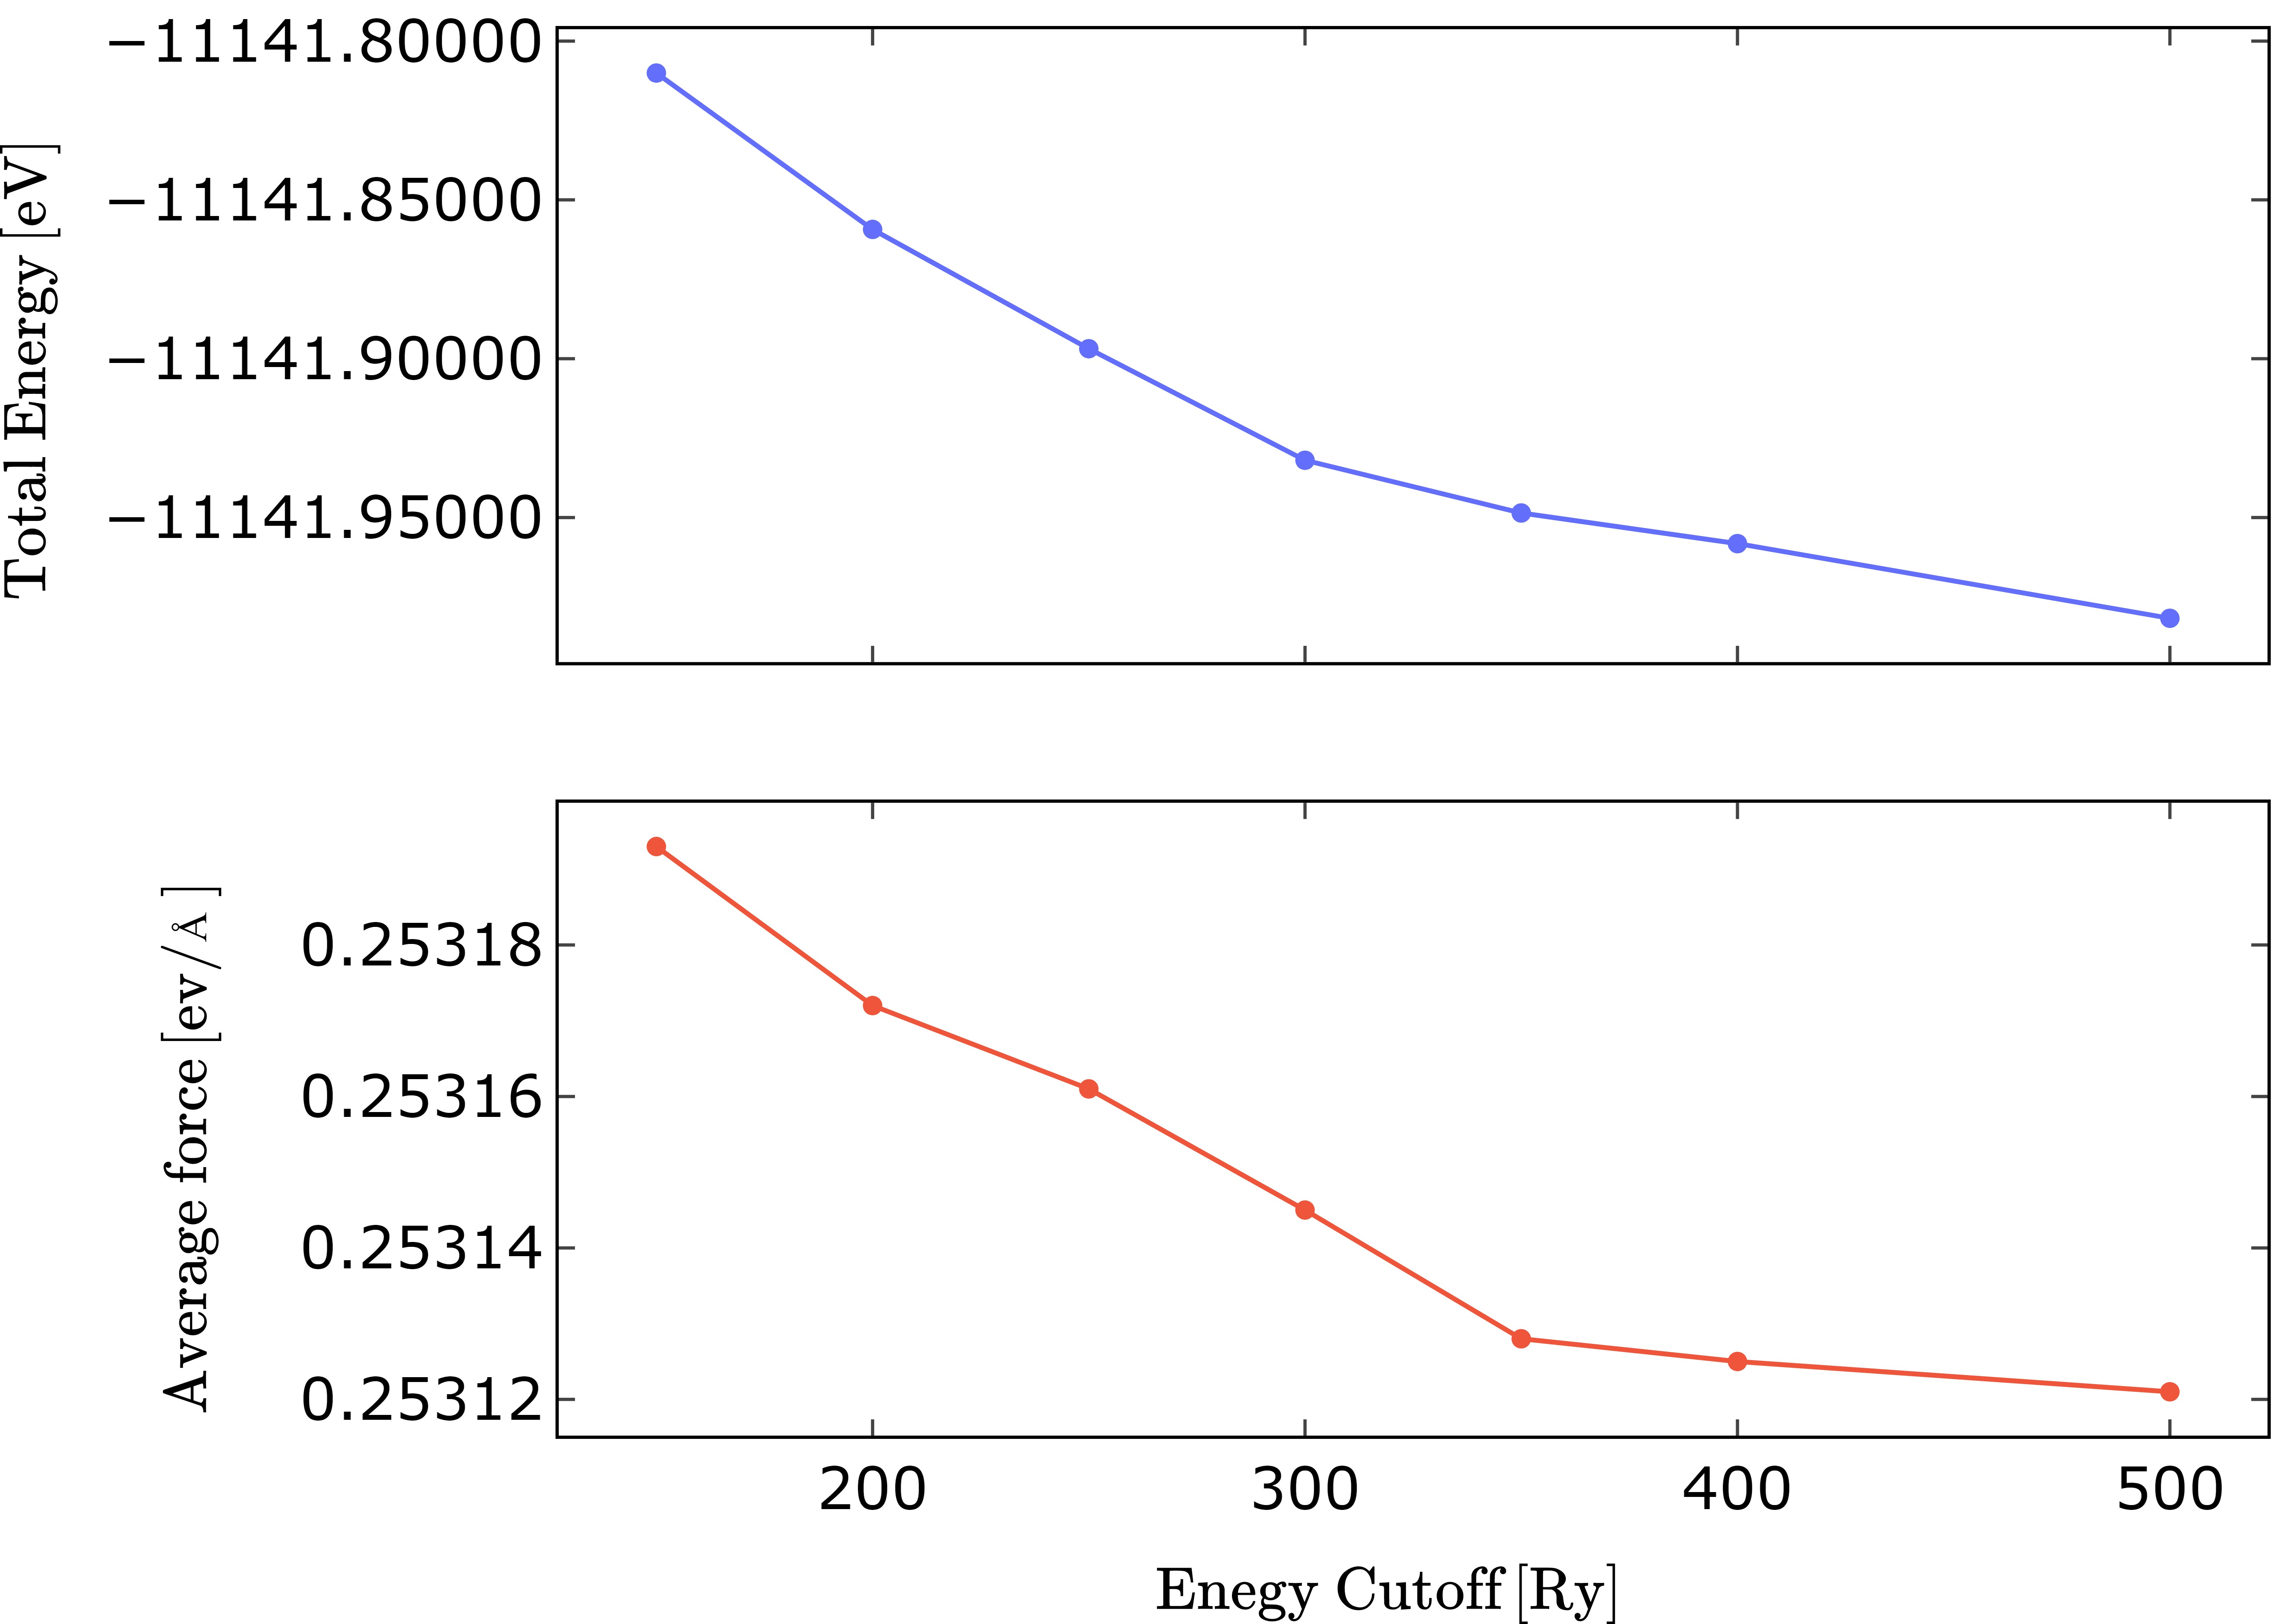
\includegraphics[width=.8\textwidth]{
      asset/cutoff_convergence.jpg
    }
  \end{center}
  \caption{Energy cutoff convergence test for the DFT training data.}
  \label{fig:dft_energy_cutoff_convergence}
\end{figure}

\begin{figure}
  \begin{center}
    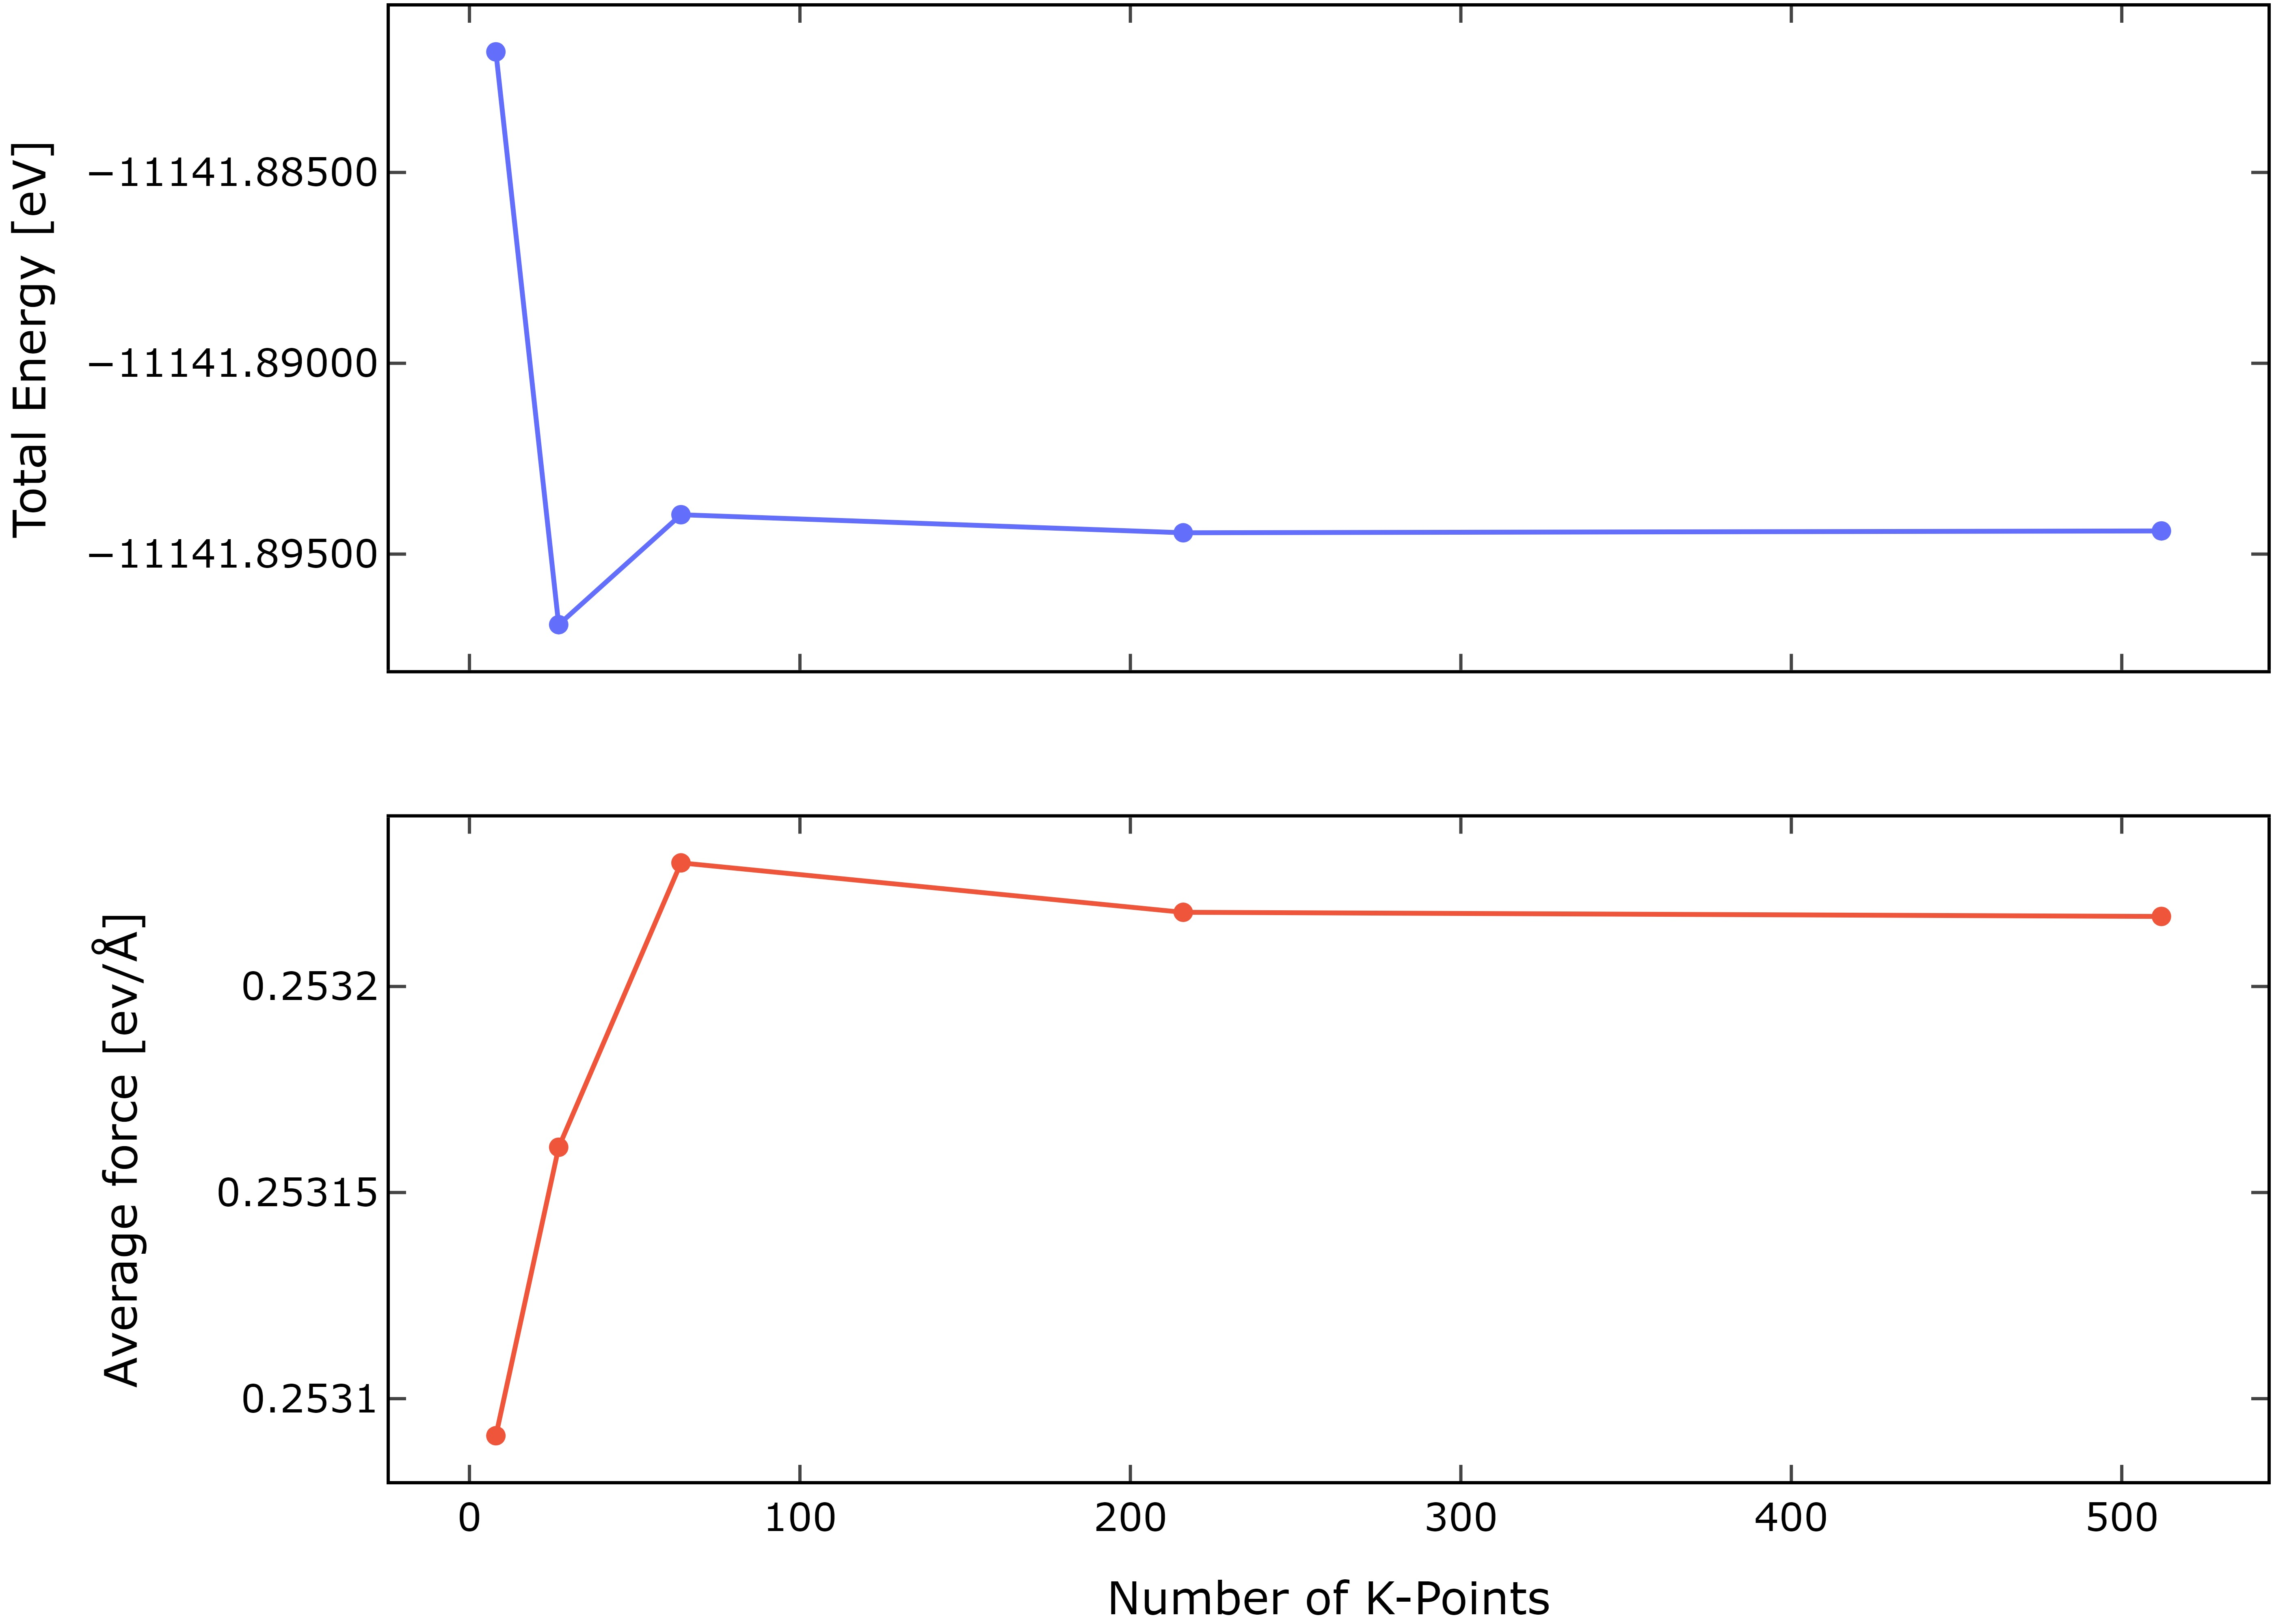
\includegraphics[width=.8\textwidth]{
      asset/kpoint_convergence.jpg
    }
  \end{center}
  \caption{K-Point convergence test for the DFT training data.}
  \label{fig:dft_kpoint_convergence}
\end{figure}

\section{Training Results}

All models were trained on dual AMD EPYC 7H12 64-Core processor machine.
Although such specs look impressive, the underlying training algorithms used
by DeepMD-kit seemd to not be optimized for CPU training and the whole process
could probably be greatly accelerated by training on GPUs. DeepMD-kit allows
to fine-tune the training process by adjusting the runtime parameters
\texttt{OMP\_NUM\_THREADS}, \texttt{TF\_INTRA\_OP\_PARALLELISM\_THREADS},
\linebreak and \texttt{TF\_INTER\_OP\_PARALLELISM\_THREADS}. Despite running
many empirical tests to arrive at the optimal values for these parameters, the
training process did not speed up significantly. The training sessions took
about $12 \, \mathrm{h}$ for the larger models and about $8 \, \mathrm{h}$ for
the smaller models.

A typical descending learning curve was observed for models trained on the
amorphous and combined datasets. When increasing the number of descriptor
neurons from $[5, 10, 20]$ (figure
\ref{fig:amorphous_5,10,20d_20,20,20f_260222622s-learning-curves}) to
$[25, 50, 100]$ (figure
\ref{fig:amorphous_25,50,100d_20,20,20f_260222622s-learning-curves}) we don't
observe significant changes in the learning curves. On the other hand, when
increasing the number of fitting neurons from $[10, 10, 10]$
(figure \ref{fig:amorphous_10,20,40d_10,10,10f_260222622s-learning-curves}) to
$[75, 75, 75]$ (figure
\ref{fig:amorphous_10,20,40d_75,75,75f_260222622s-learning-curves}) we can
observe a very slight divergence of training error and validation error with
increasing training step. We can see from the error evaluation plot for
descriptor neurons (figure \ref{fig:descriptor_energy_error_evaluation}) that
the energy error slightly decreases with increasing number of descriptor
neurons, although this effect is negligible. The effect of increasing energy
error with increasing number of fitting neurons can also be observed in the
error evaluation plot for fitting neurons (figure
\ref{fig:fitting_energy_error_evaluation}). Both of these effects are much
more pronounced for the crystalline dataset, where data scarcity is a
significant concern. Although, the crystalline system should be the simplest
to model, the shortage of data plays a major role here, which can be observed
in the learning curves and in the energy error evaluation plots.
The predictions for the crystalline system get outstandingly better when
increasing the number of descriptor neurons from $[5, 10, 20]$ (figure
\ref{fig:crystalline_5,10,20d_20,20,20f_260222622s-learning-curves}) to
$[25, 50, 100]$ (figure
\ref{fig:crystalline_25,50,100d_20,20,20f_260222622s-learning-curves}). This
might have several reasons. First, the higher number of descriptor neurons
make the model more flexible and more unlikely to underfit on low data
volumes. The second reason might be that the higher number of descriptor
neurons allows the model to better capture the underlying structure of the
sillicon system, since this effect is observable for the amorphous and
combined systems as well. While the number of descriptor neurons correlates
positively with inference quality, the opposite is true for the number of
fitting neurons. When increasing fitting neurons from $[10, 10, 10]$
(figure \ref{fig:crystalline_10,20,40d_10,10,10f_260222622s-learning-curves})
to $[75, 75, 75]$
(figure \ref{fig:crystalline_10,20,40d_75,75,75f_260222622s-learning-curves})
we observe the energy error increases, and the dissonance of training error
and validation error broadens. In this case, the model architecute is too
complex and overfits on the small sample of training data. We can also see
the discussed effects in the error evaluation plots for descriptor neurons
and fitting neurons (figures \ref{fig:descriptor_energy_error_evaluation} and
\ref{fig:fitting_energy_error_evaluation} respectively).

The force errors in all of the learning curves seem to converge relatively
quickly for all of the training sessions. Further training steps don't seem to
significantly improve the prediction quality and may even lead to worse
predictions. This is most likely due to the fact that the forces are very
close to zero for most of the training data, and the models are able to learn
the small deviations from zero very quickly. The increase in force error over
time is caused by the fact that the weights of the objective function are
initially set to prioritize the force error over the energy error and then
gradually shift towards prioritizing energy error over force error, as already
discussed.

\begin{figure}
  \begin{center}
    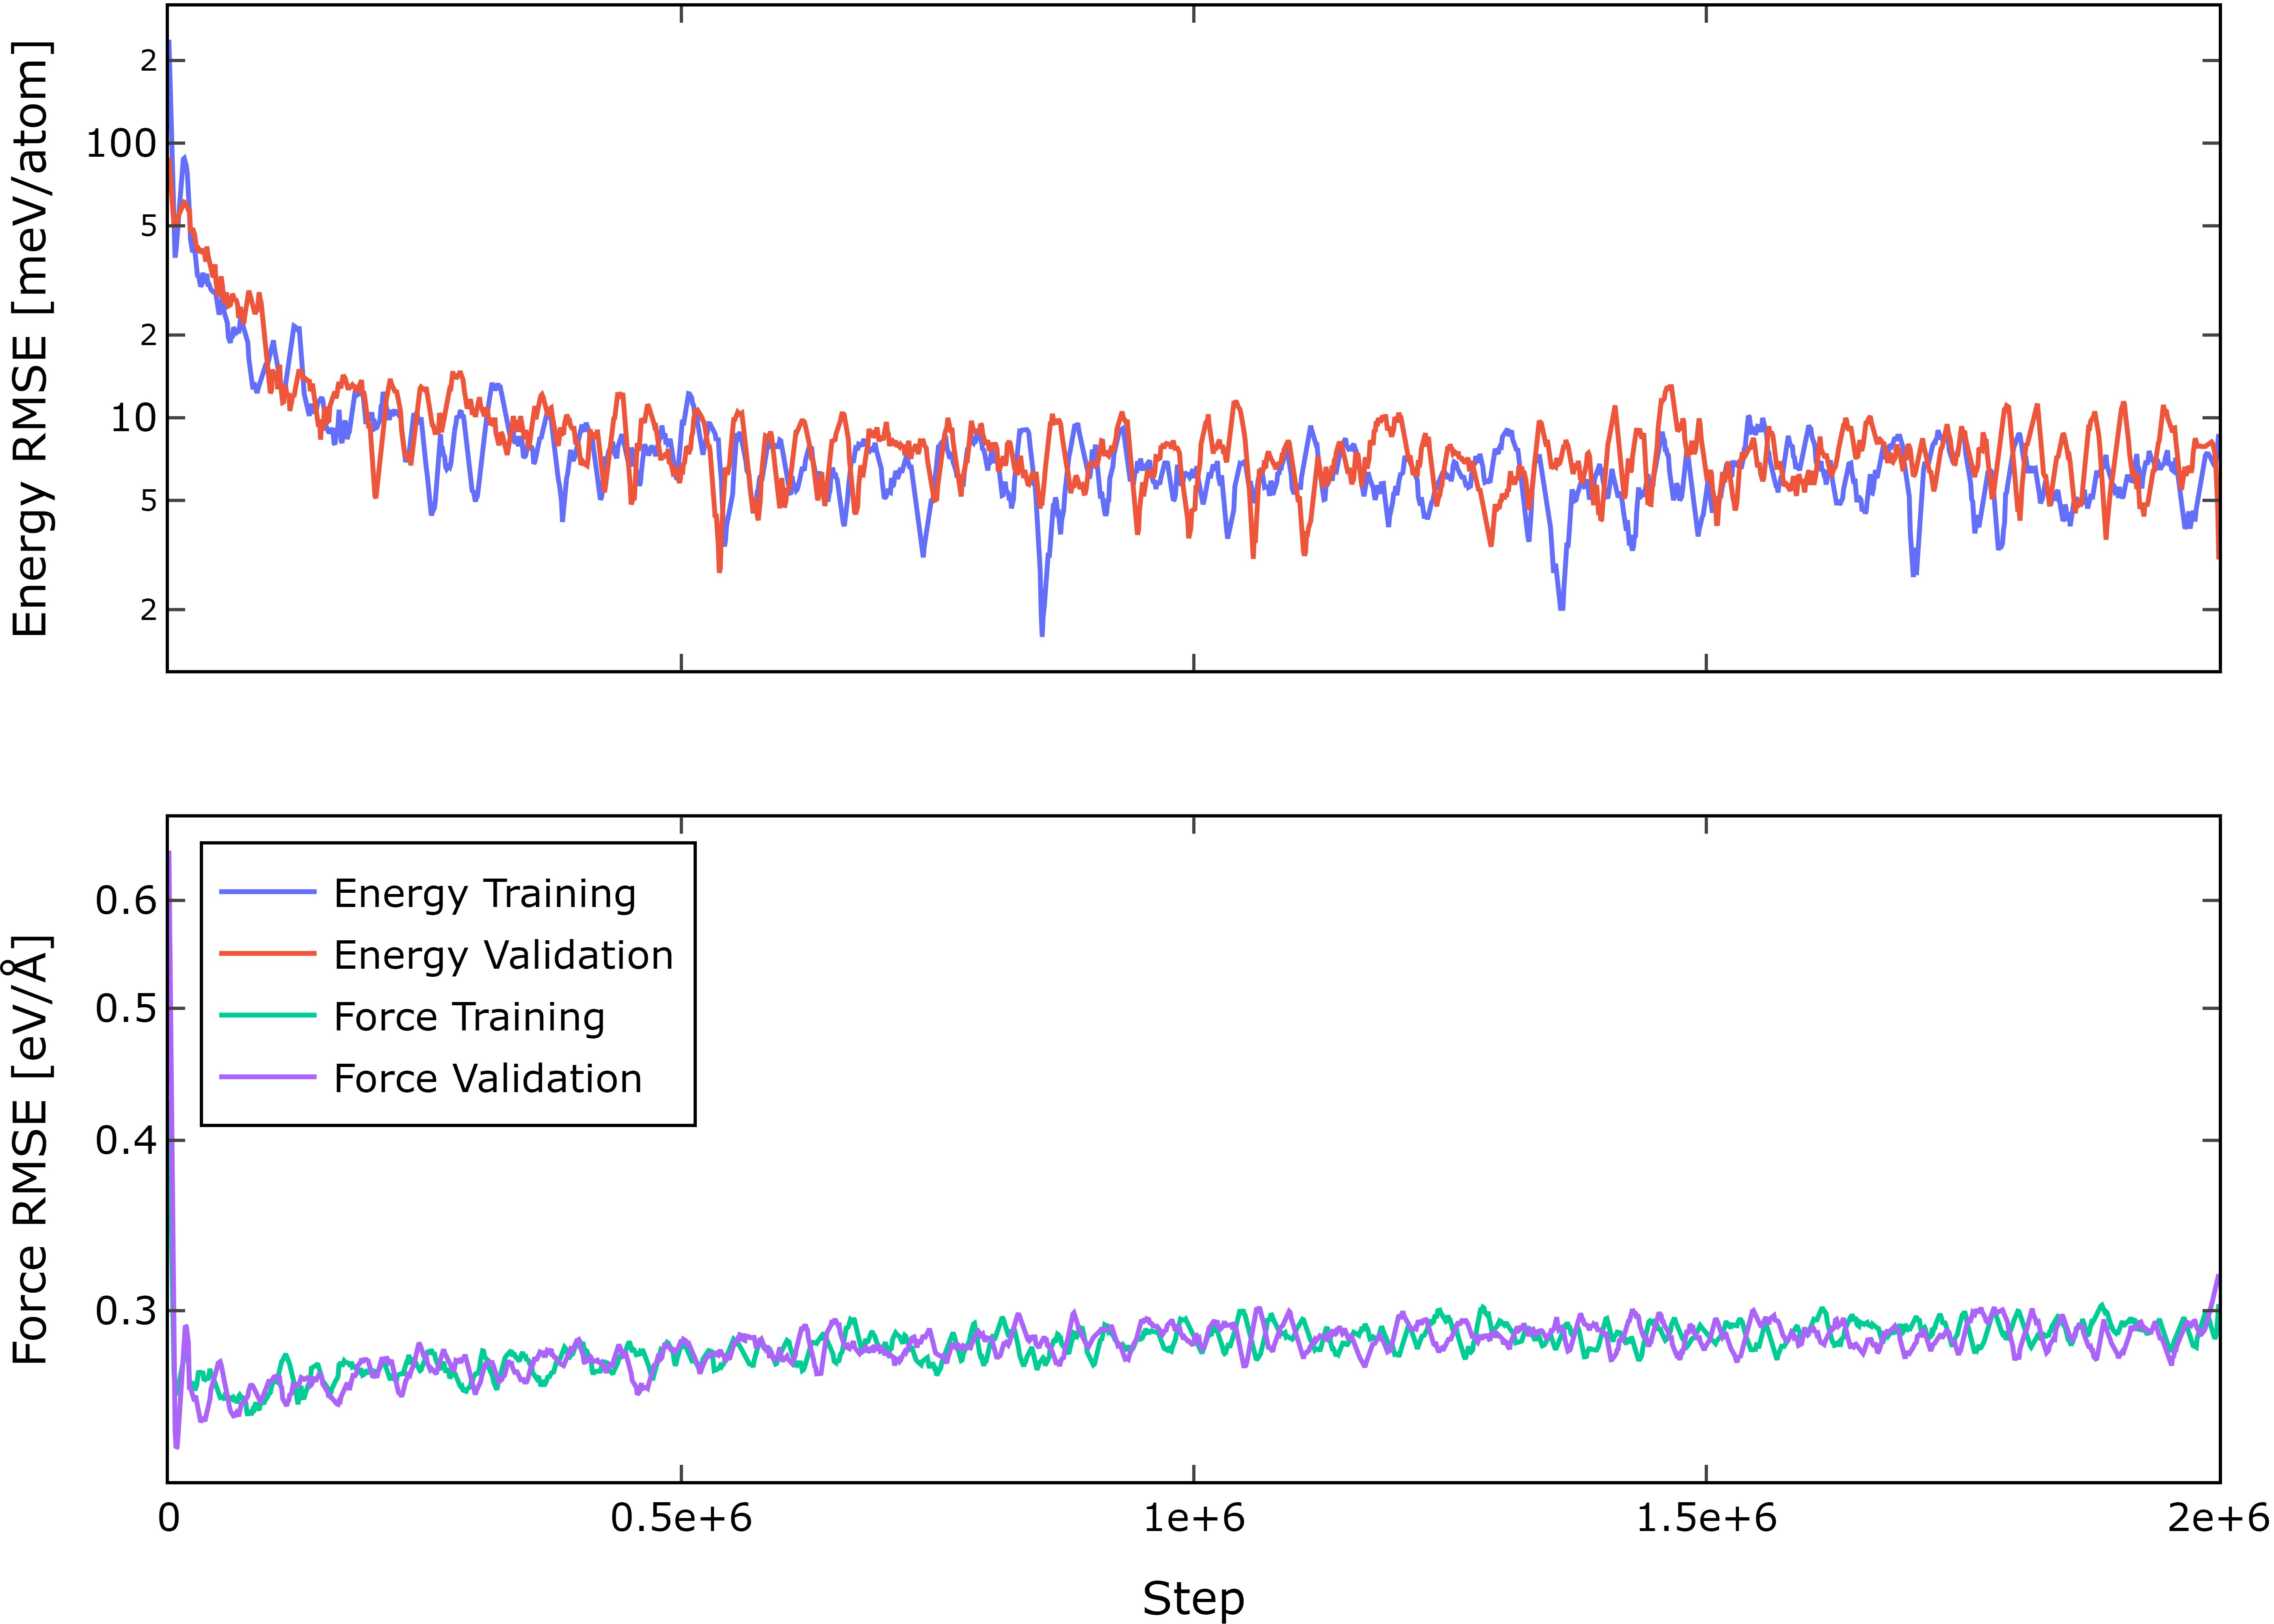
\includegraphics[width=.8\textwidth]{
      asset/amorphous_5,10,20d_20,20,20f_260222622s_energy_force_l_curve.jpg
    }
  \end{center}
  \caption{Learning curves for model \texttt{amorphous\_5,10,20d\_20,20,20f\_260222622s}.}
  \label{fig:amorphous_5,10,20d_20,20,20f_260222622s-learning-curves}
\end{figure}

\begin{figure}
  \begin{center}
    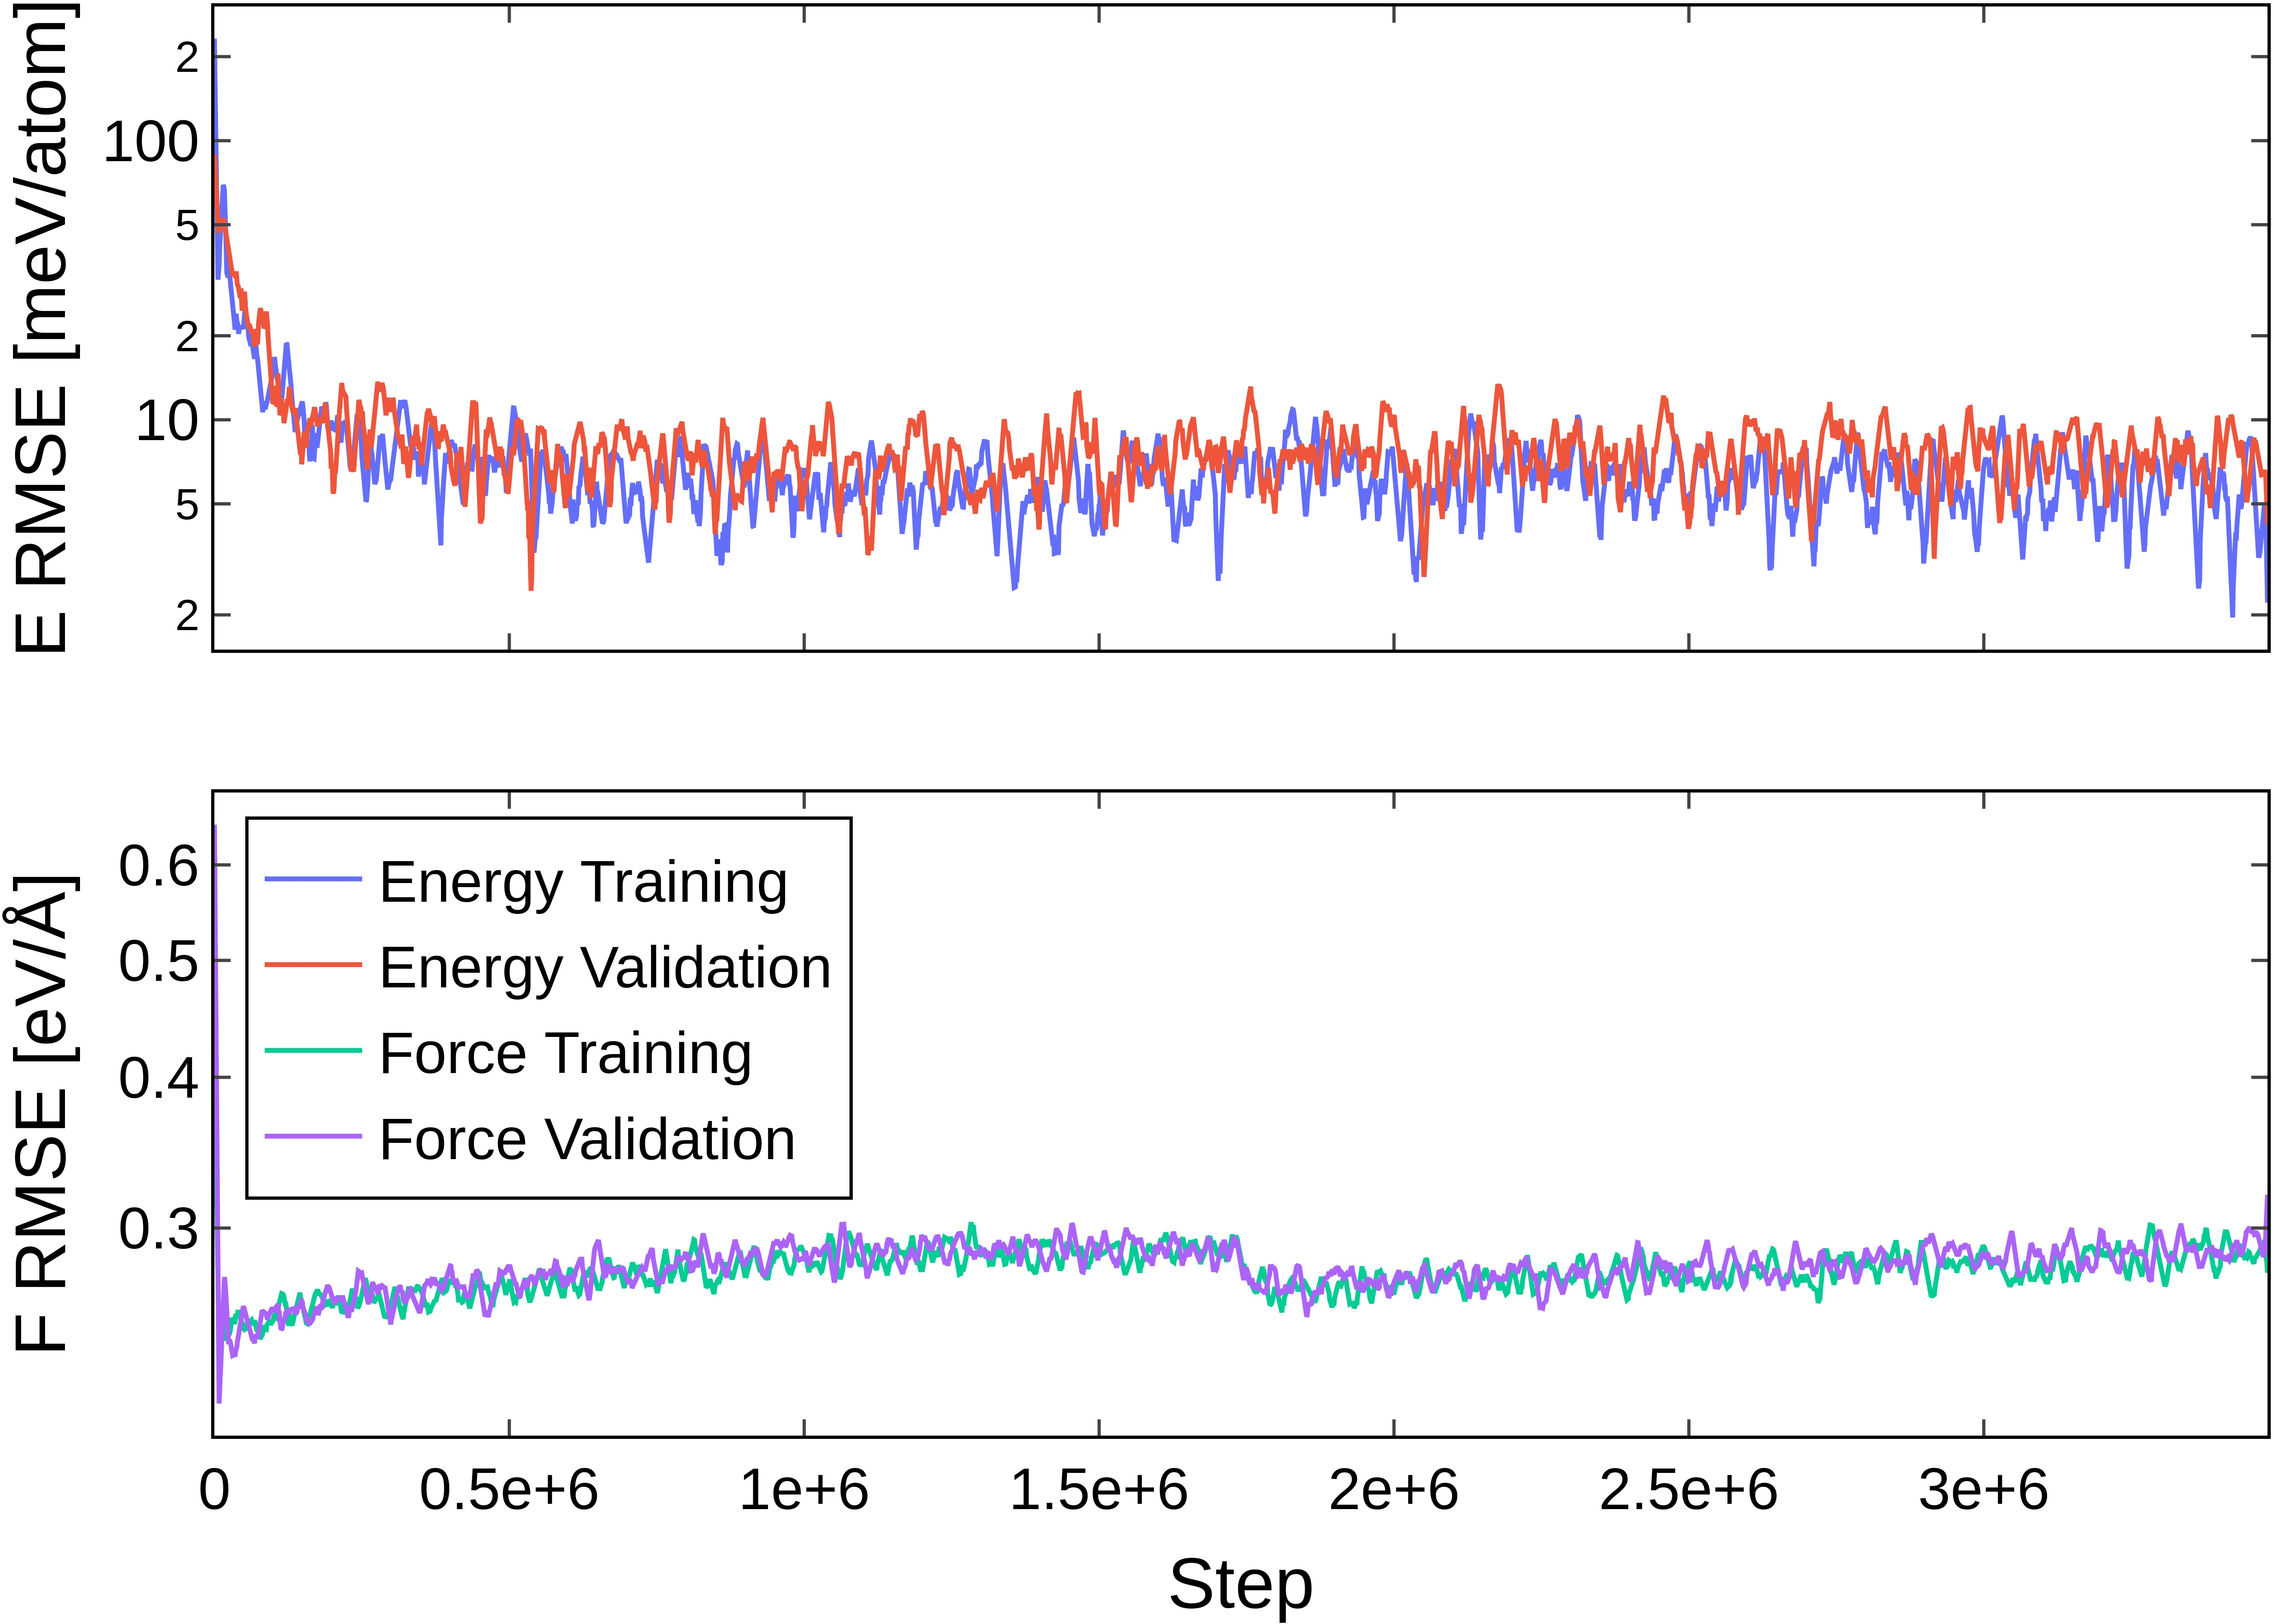
\includegraphics[width=.8\textwidth]{
      asset/amorphous_25,50,100d_20,20,20f_260222622s_energy_force_l_curve.jpg
    }
  \end{center}
  \caption{Learning curves for model \texttt{amorphous\_25,50,100d\_20,20,20f\_260222622s}.}
  \label{fig:amorphous_25,50,100d_20,20,20f_260222622s-learning-curves}
\end{figure}


\begin{figure}
  \begin{center}
    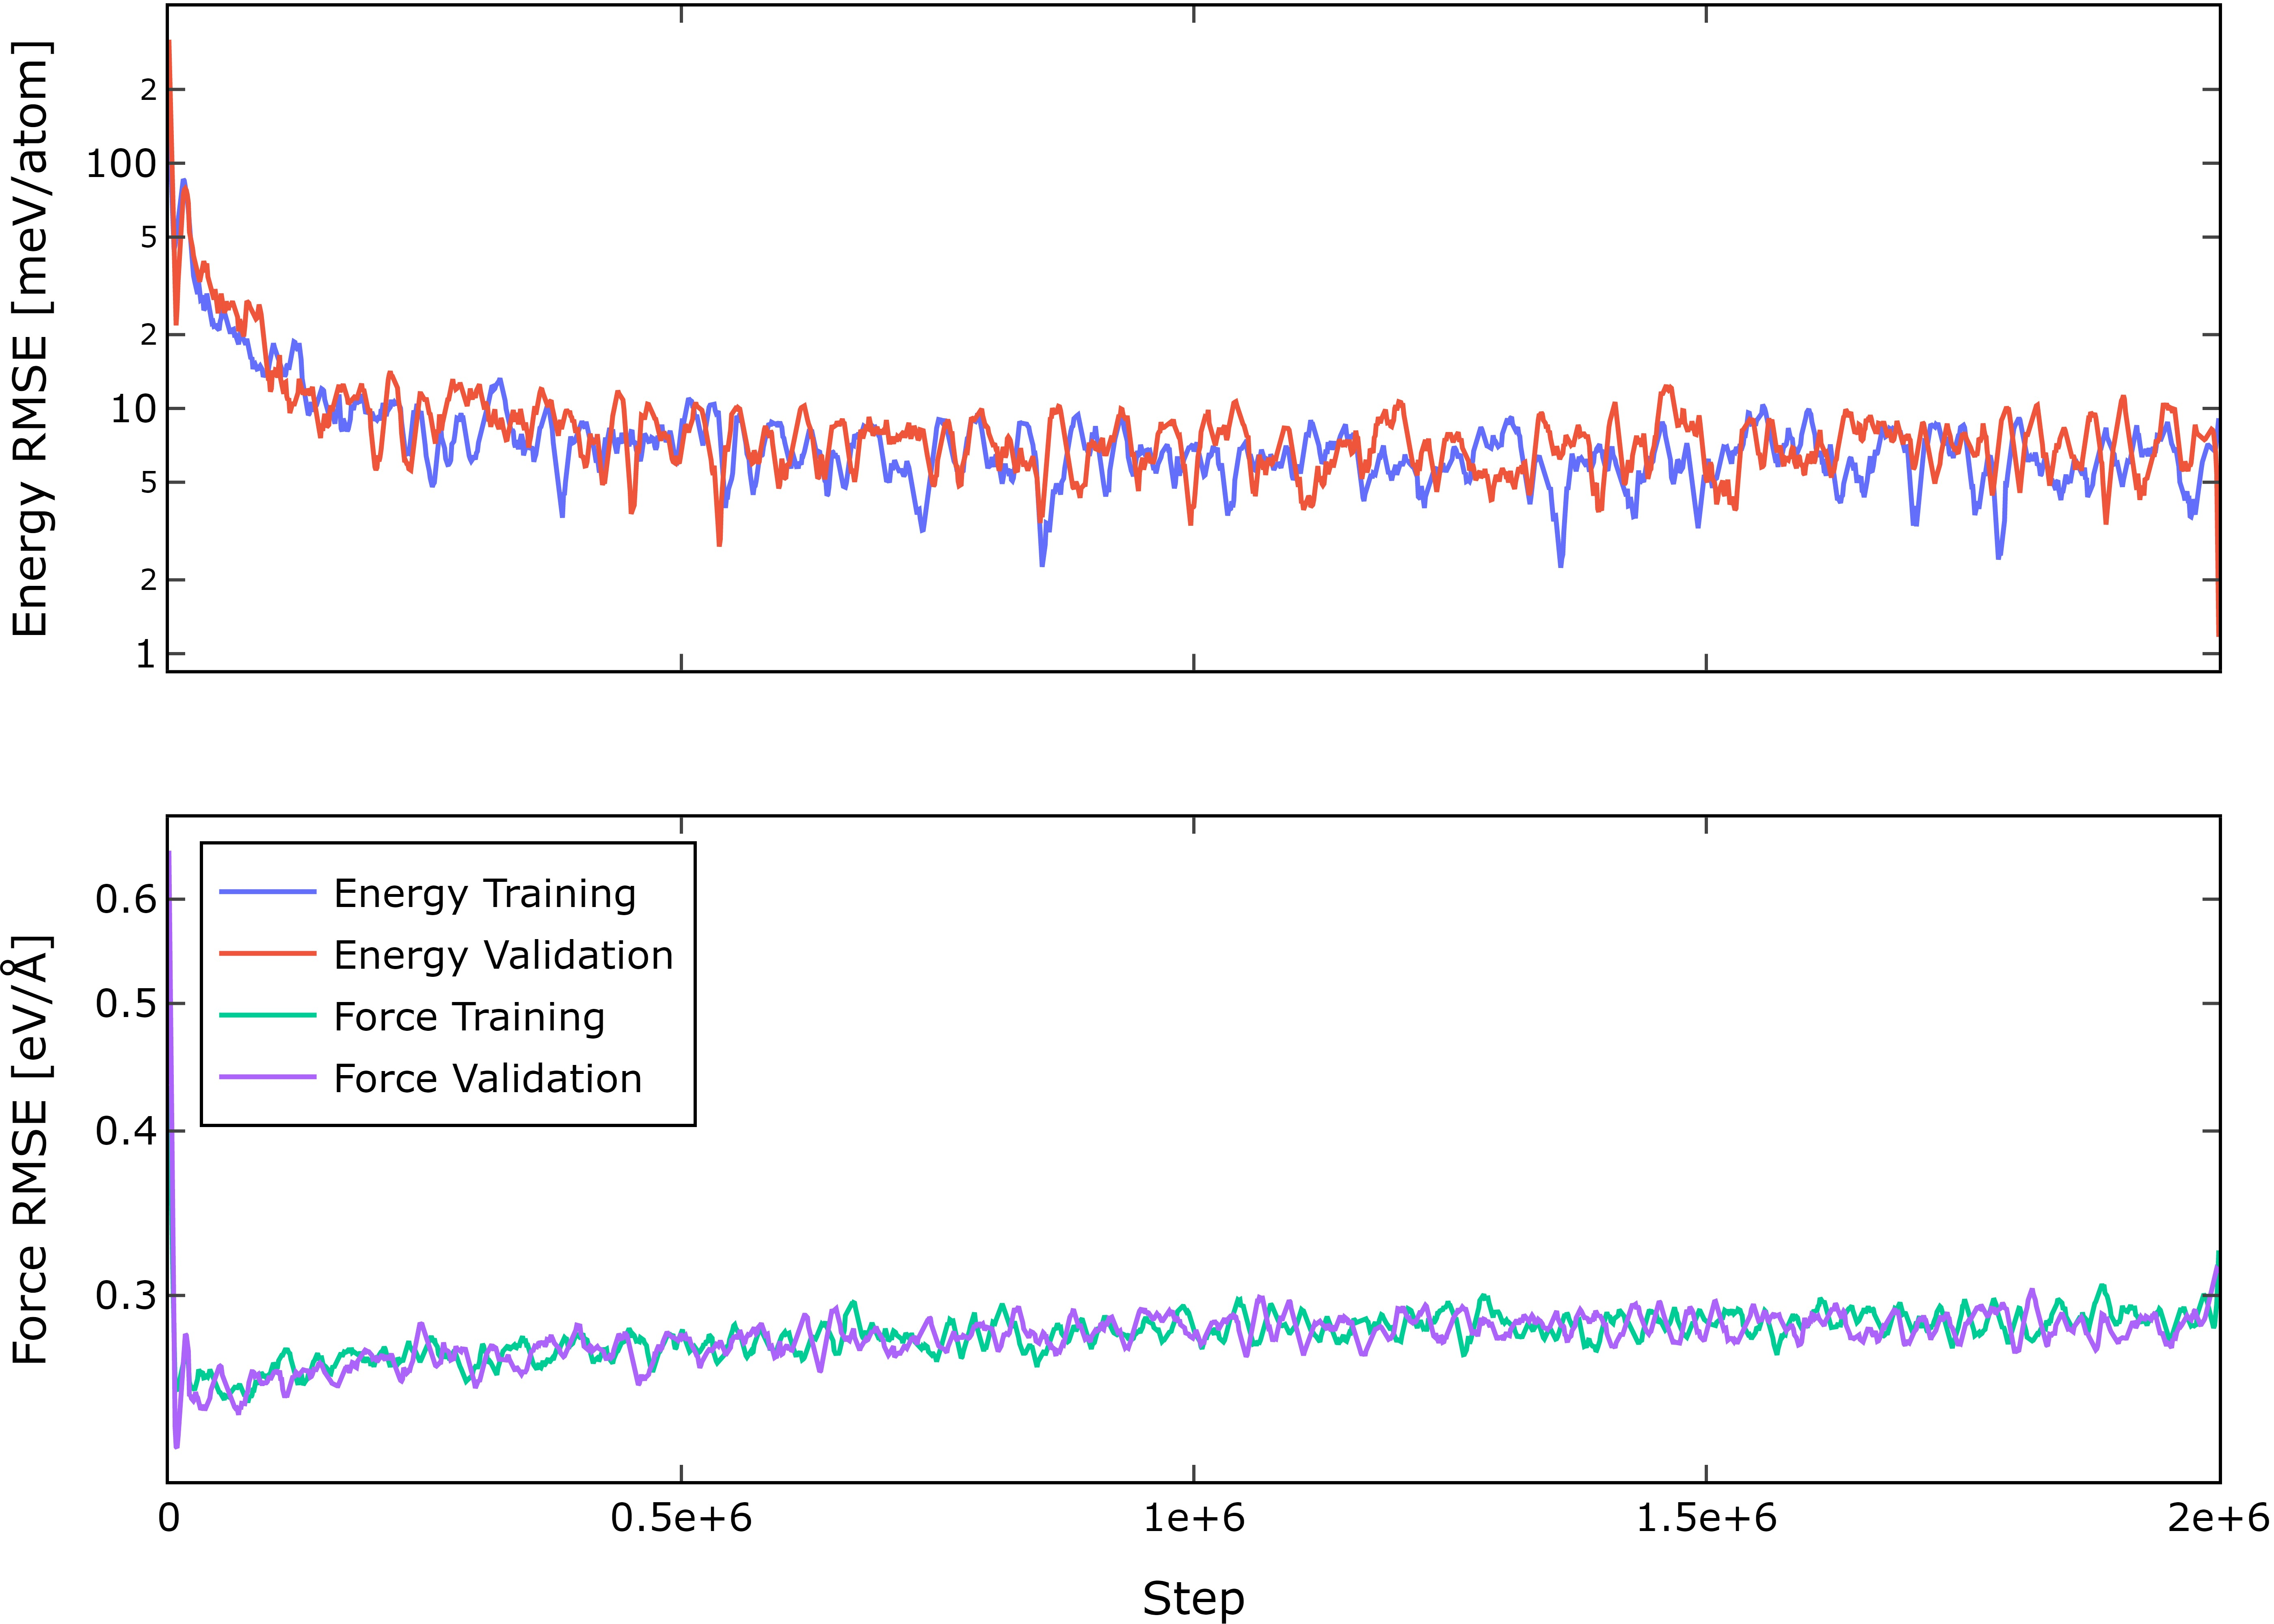
\includegraphics[width=.8\textwidth]{
      asset/amorphous_10,20,40d_10,10,10f_260222622s_energy_force_l_curve.jpg
    }
  \end{center}
  \caption{Learning curves for model \texttt{amorphous\_10,20,40d\_10,10,10f\_260222622s}.}
  \label{fig:amorphous_10,20,40d_10,10,10f_260222622s-learning-curves}
\end{figure}

\begin{figure}
  \begin{center}
    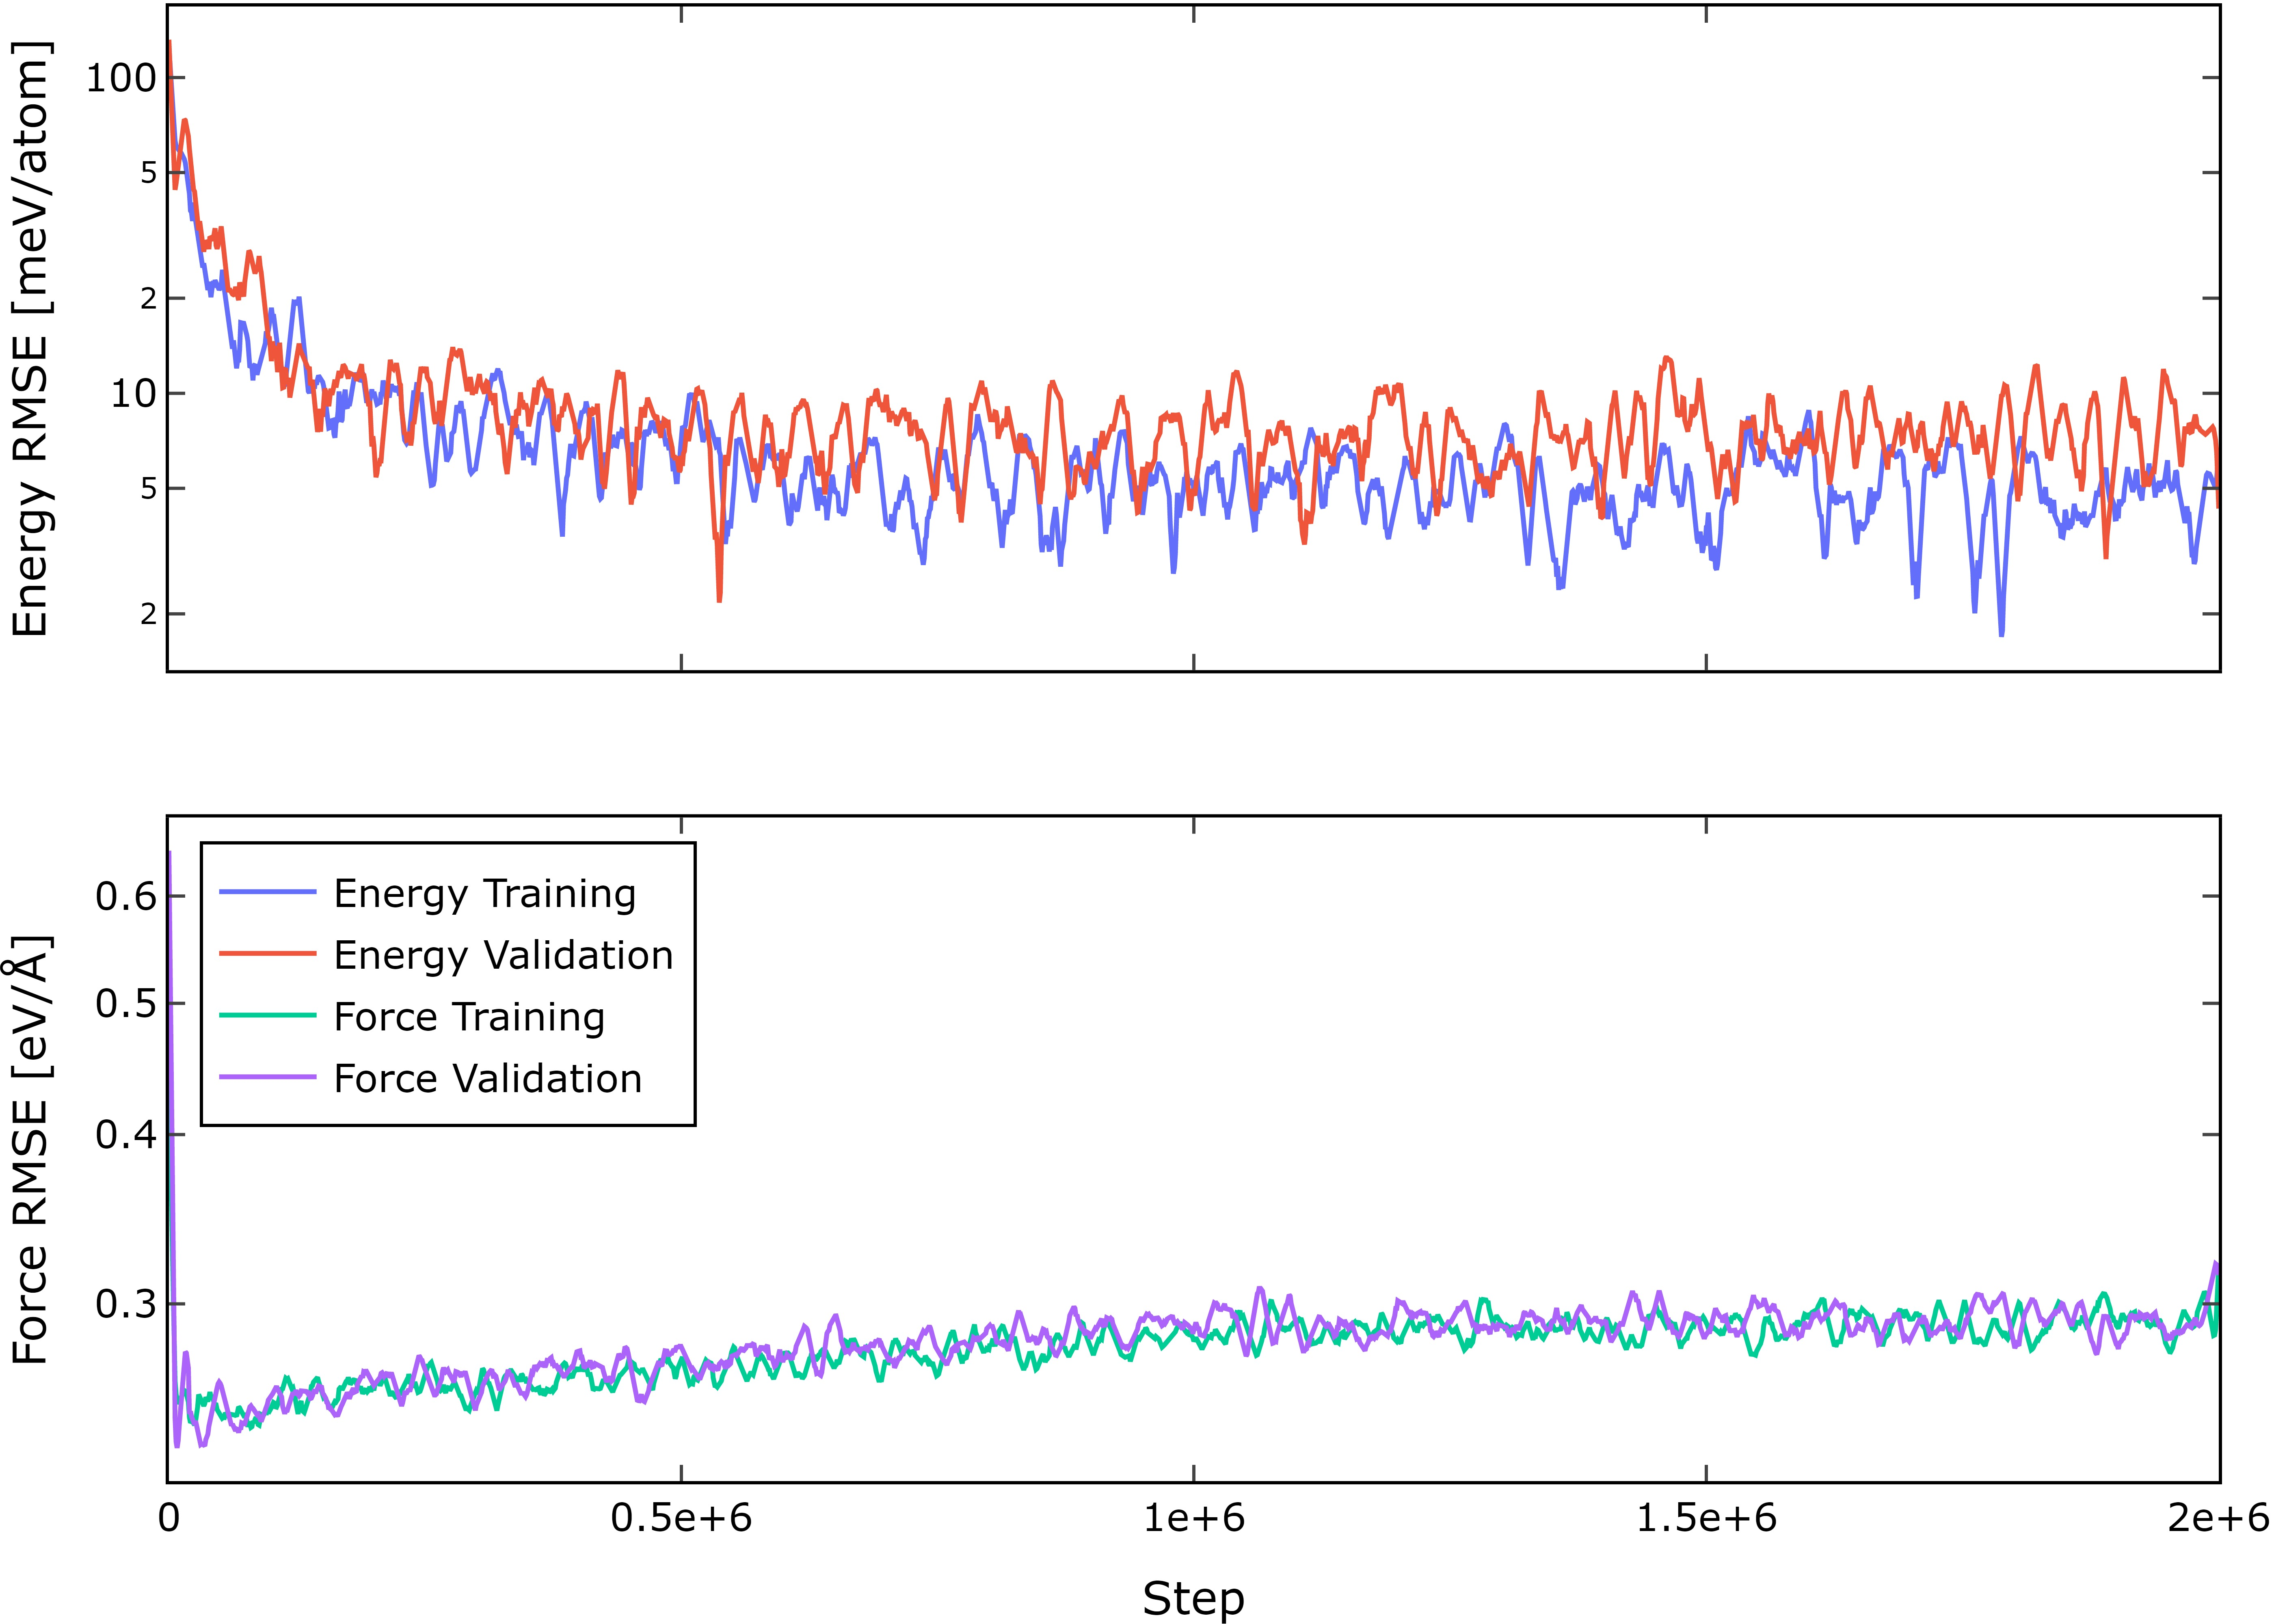
\includegraphics[width=.8\textwidth]{
      asset/amorphous_10,20,40d_75,75,75f_260222622s_energy_force_l_curve.jpg
    }
  \end{center}
  \caption{Learning curves for model \texttt{amorphous\_10,20,40d\_75,75,75f\_260222622s}.}
  \label{fig:amorphous_10,20,40d_75,75,75f_260222622s-learning-curves}
\end{figure}

\begin{figure}
  \begin{center}
    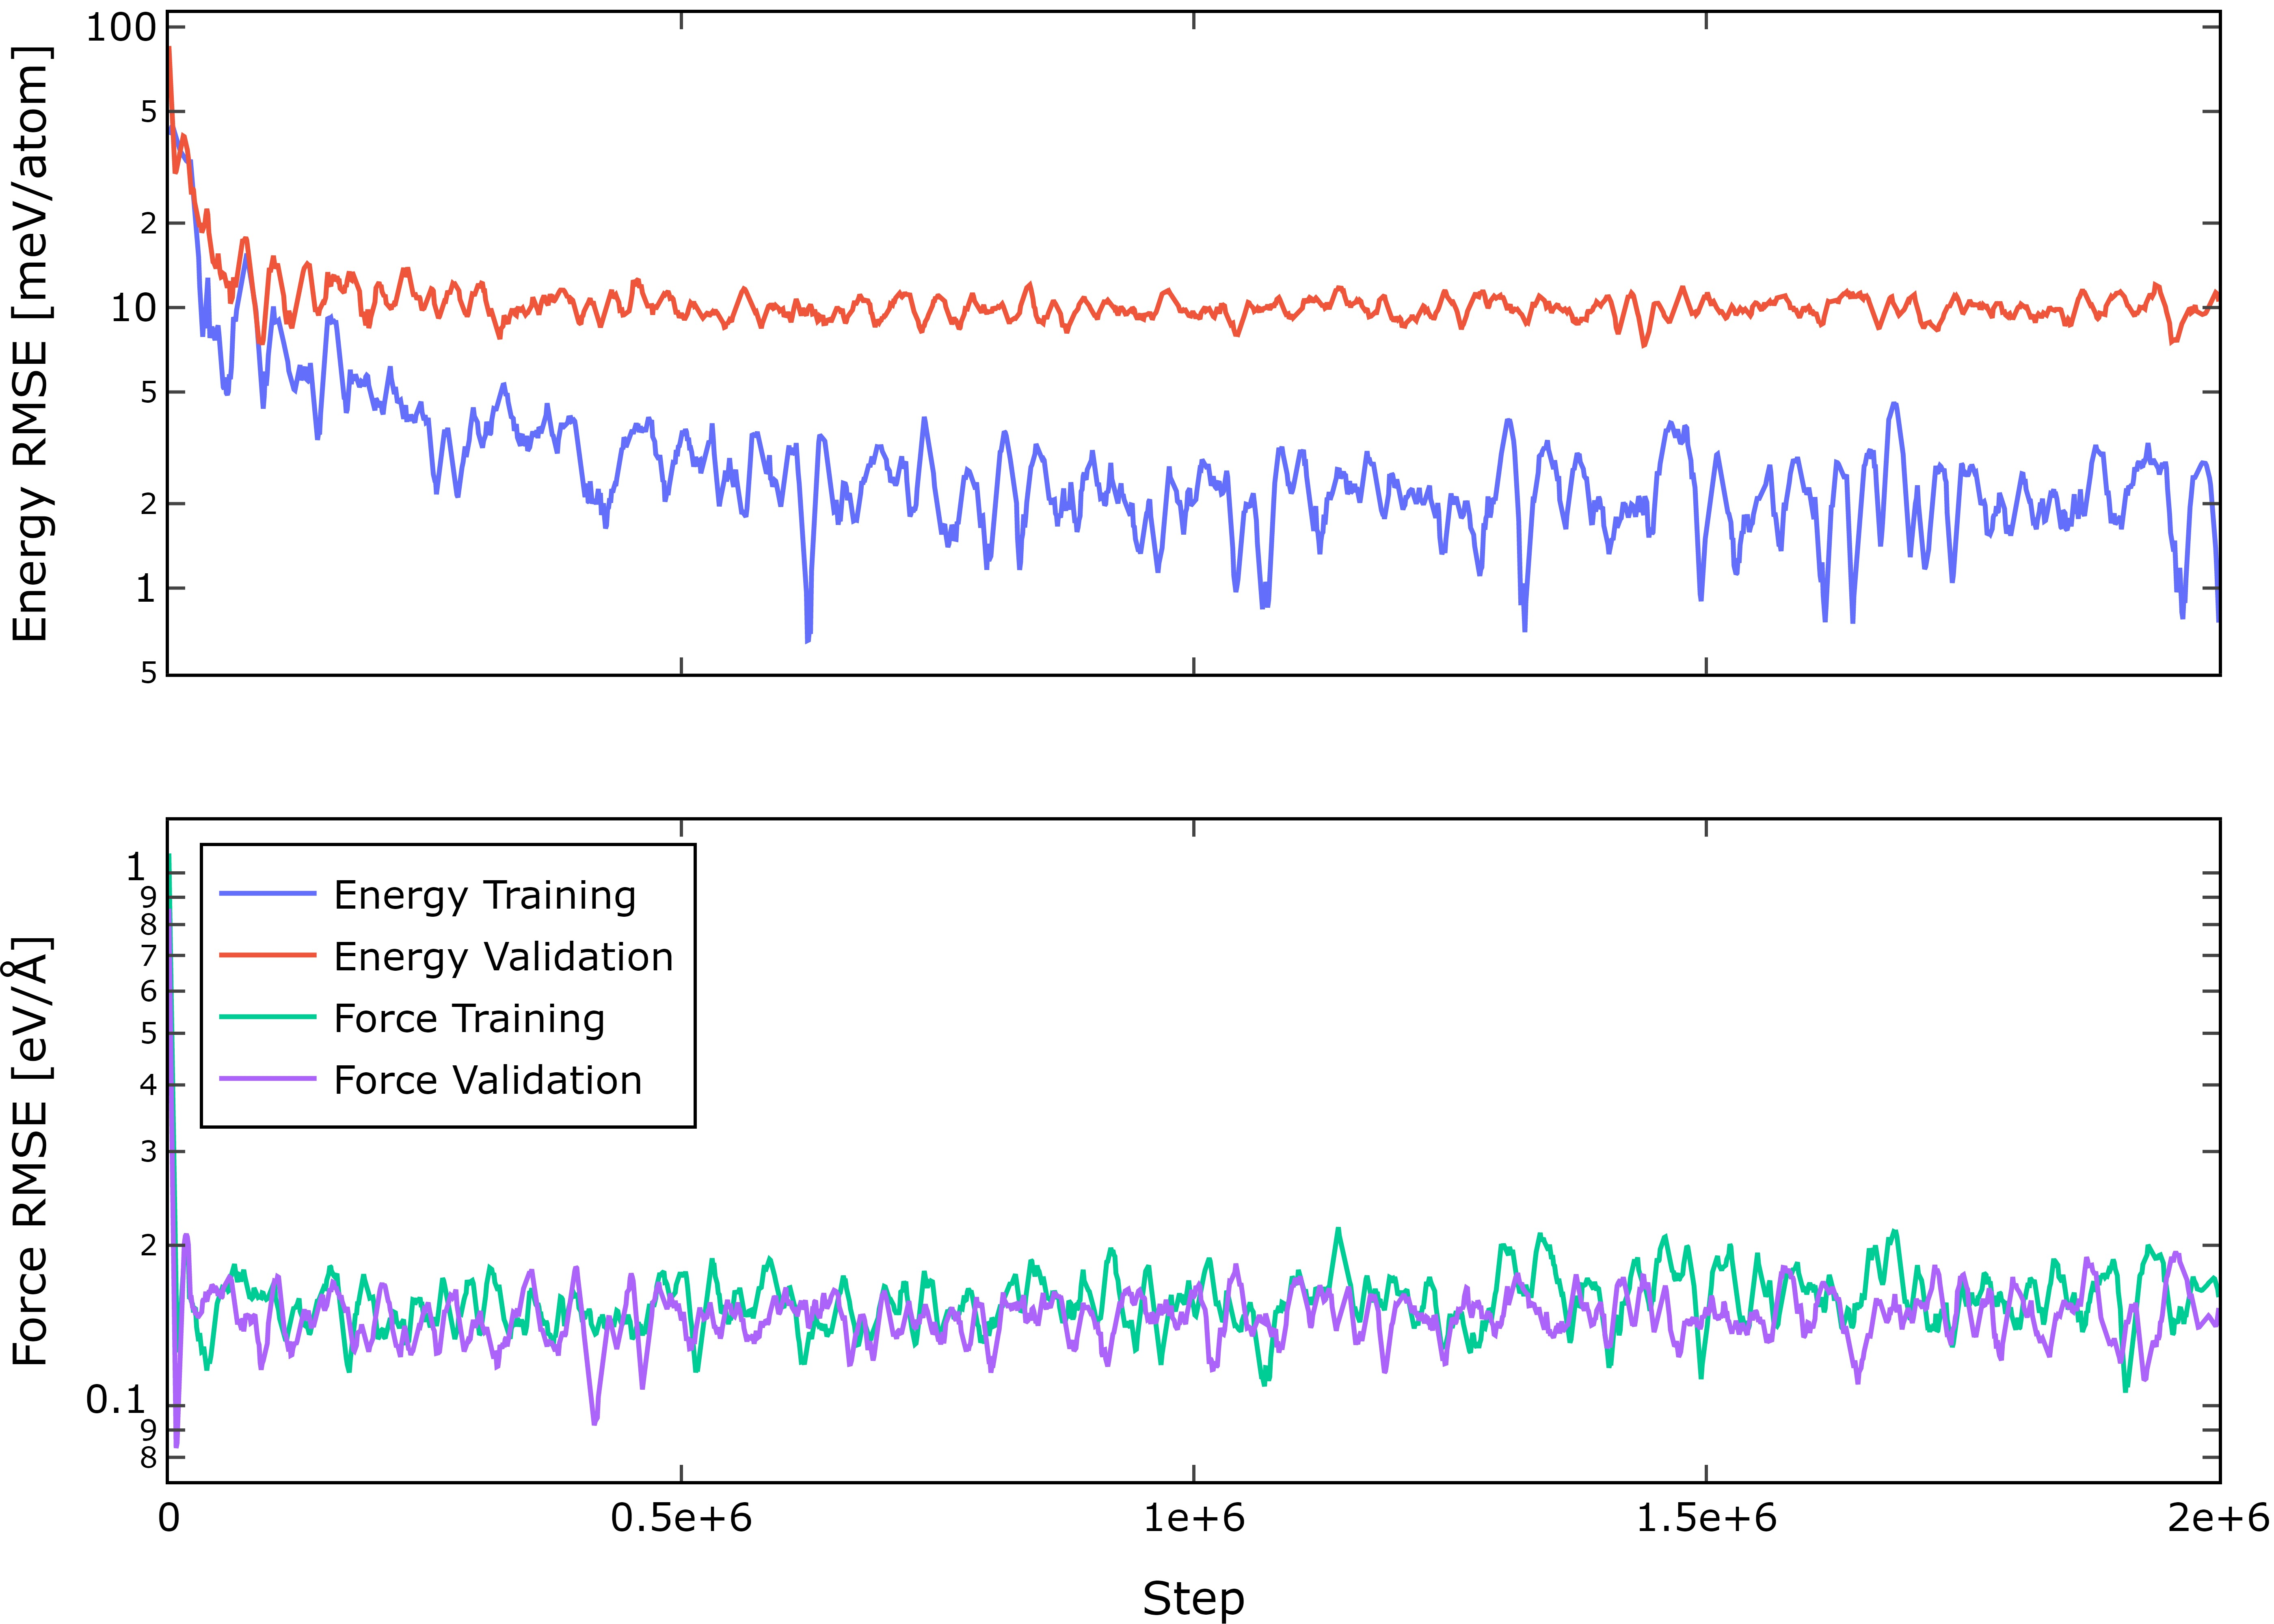
\includegraphics[width=.8\textwidth]{
      asset/crystalline_5,10,20d_20,20,20f_260222622s_energy_force_l_curve.jpg
    }
  \end{center}
  \caption{Learning curves for model \texttt{crystalline\_5,10,20d\_20,20,20f\_260222622s}.}
  \label{fig:crystalline_5,10,20d_20,20,20f_260222622s-learning-curves}
\end{figure}

\begin{figure}
  \begin{center}
    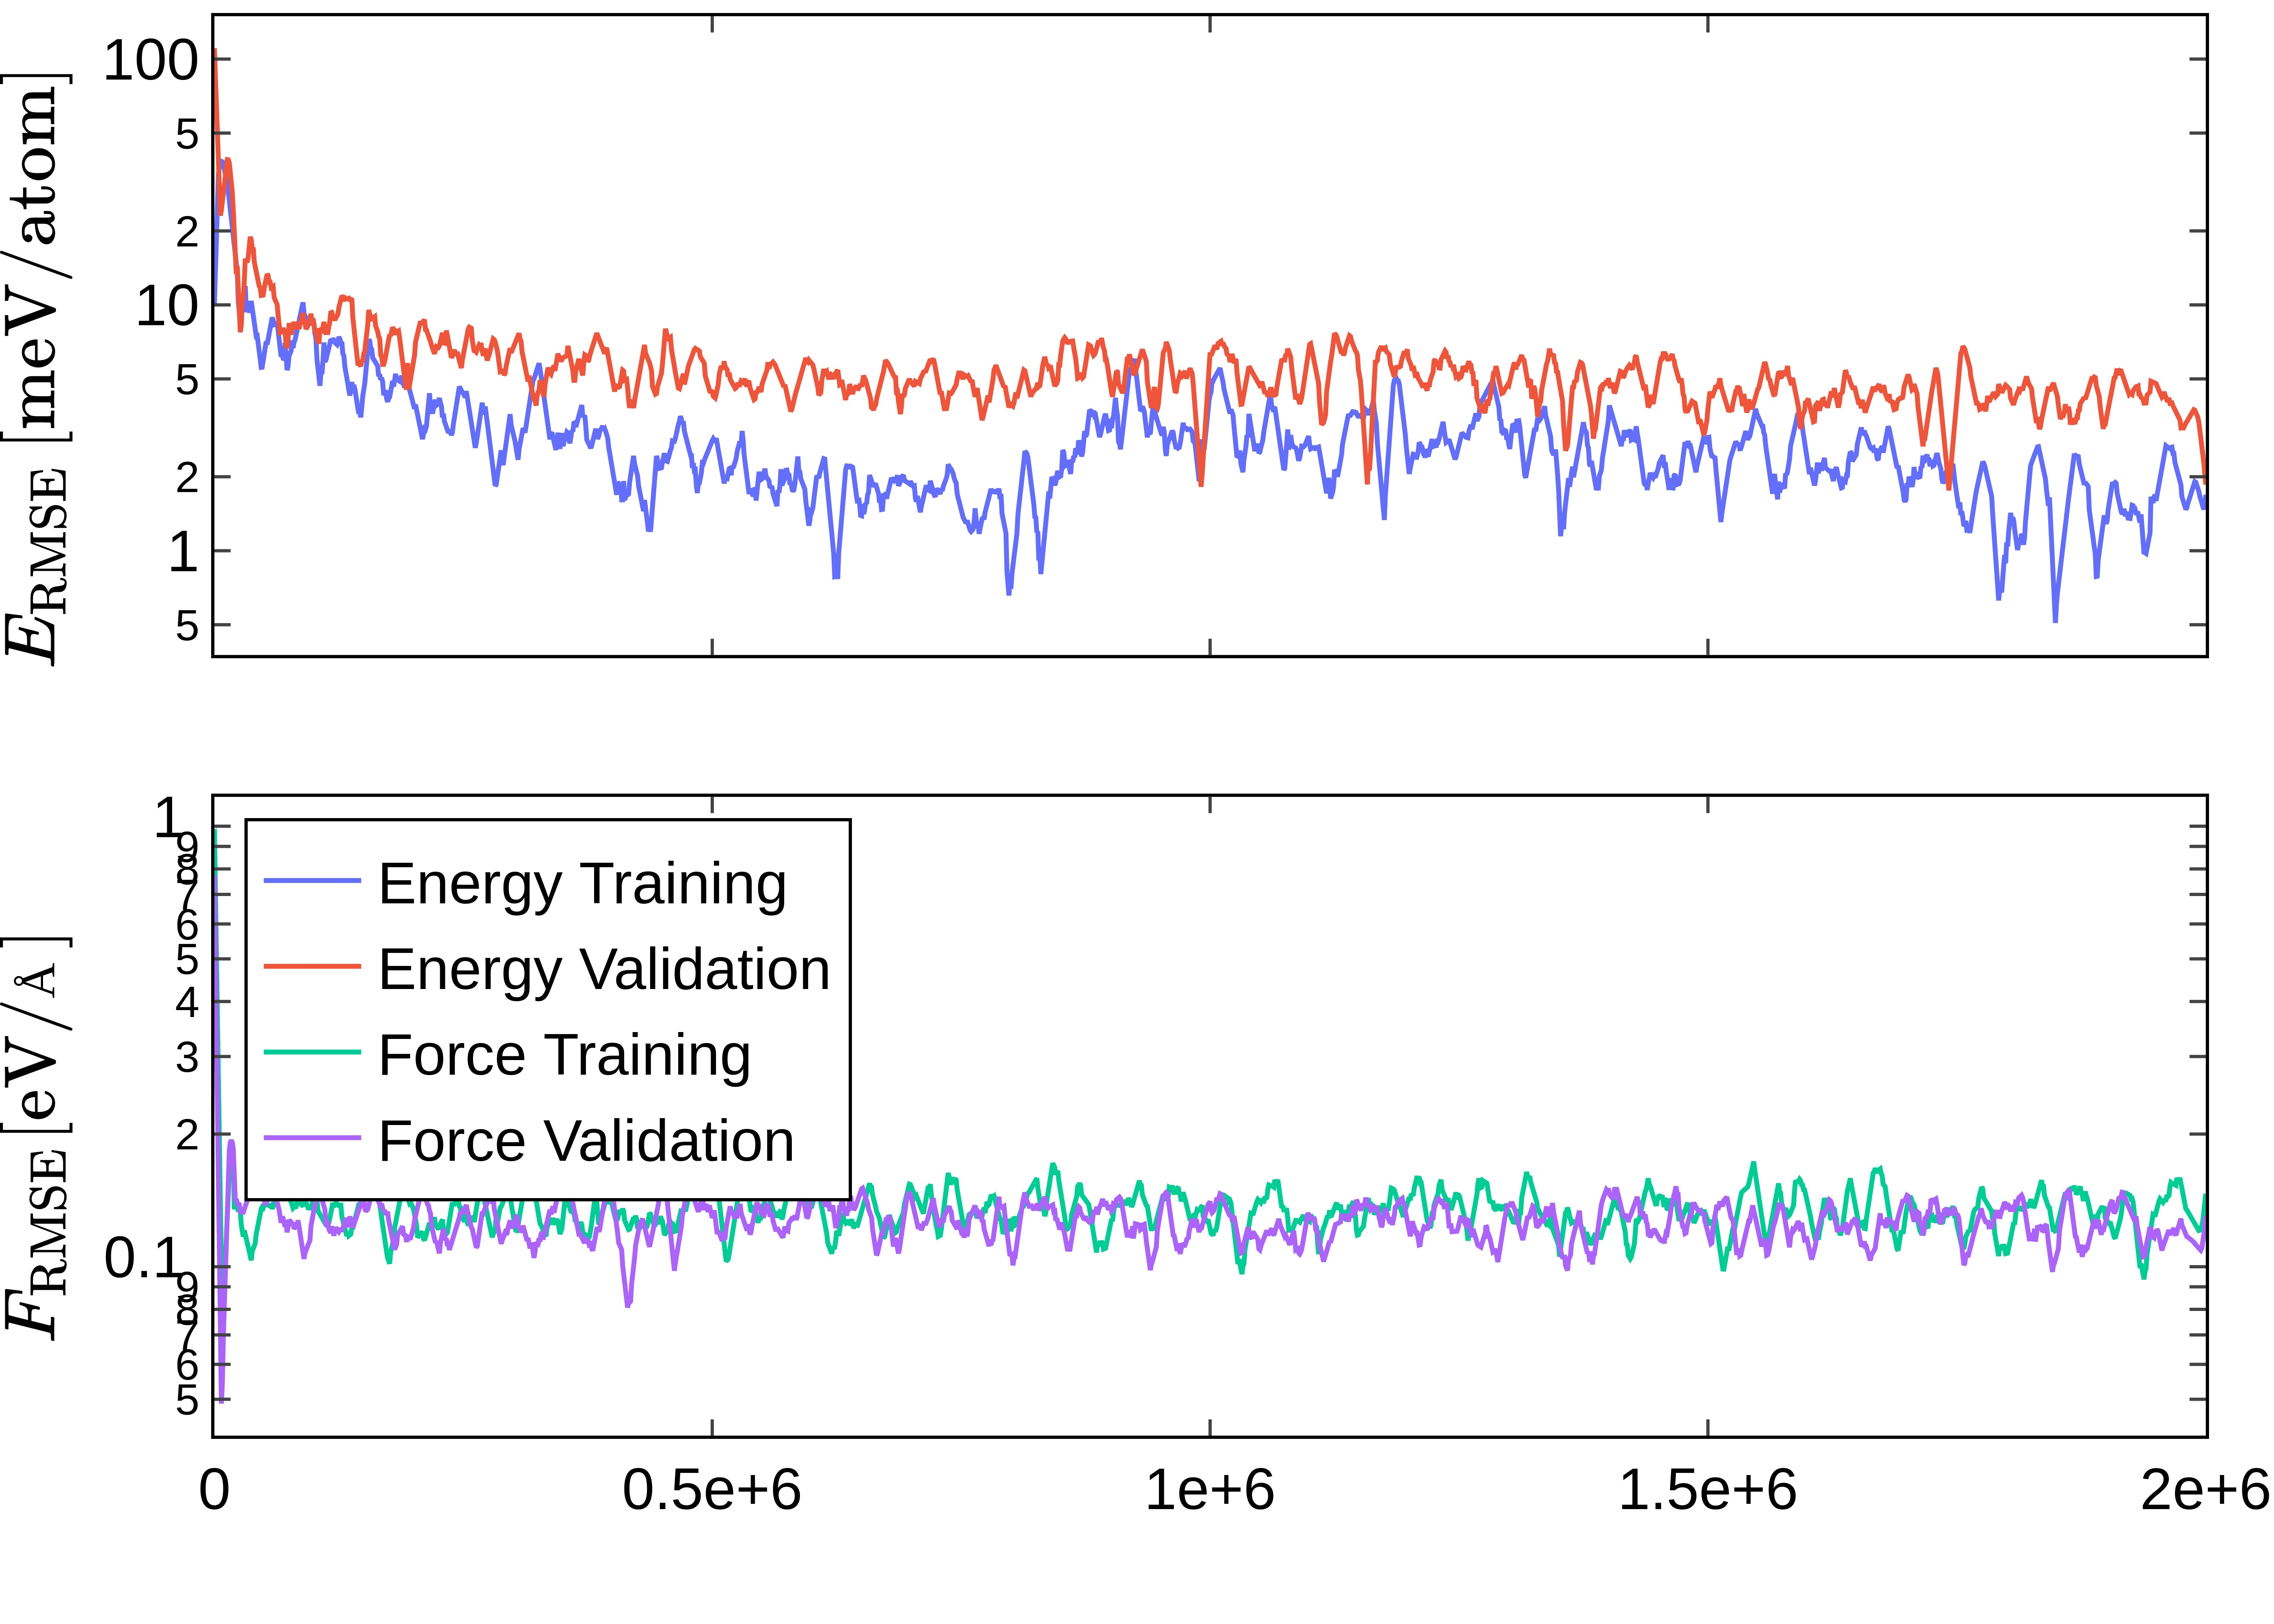
\includegraphics[width=.8\textwidth]{
      asset/crystalline_25,50,100d_20,20,20f_260222622s_energy_force_l_curve.jpg
    }
  \end{center}
  \caption{Learning curves for model \texttt{crystalline\_25,50,100d\_20,20,20f\_260222622s}.}
  \label{fig:crystalline_25,50,100d_20,20,20f_260222622s-learning-curves}
\end{figure}

\begin{figure}
  \begin{center}
    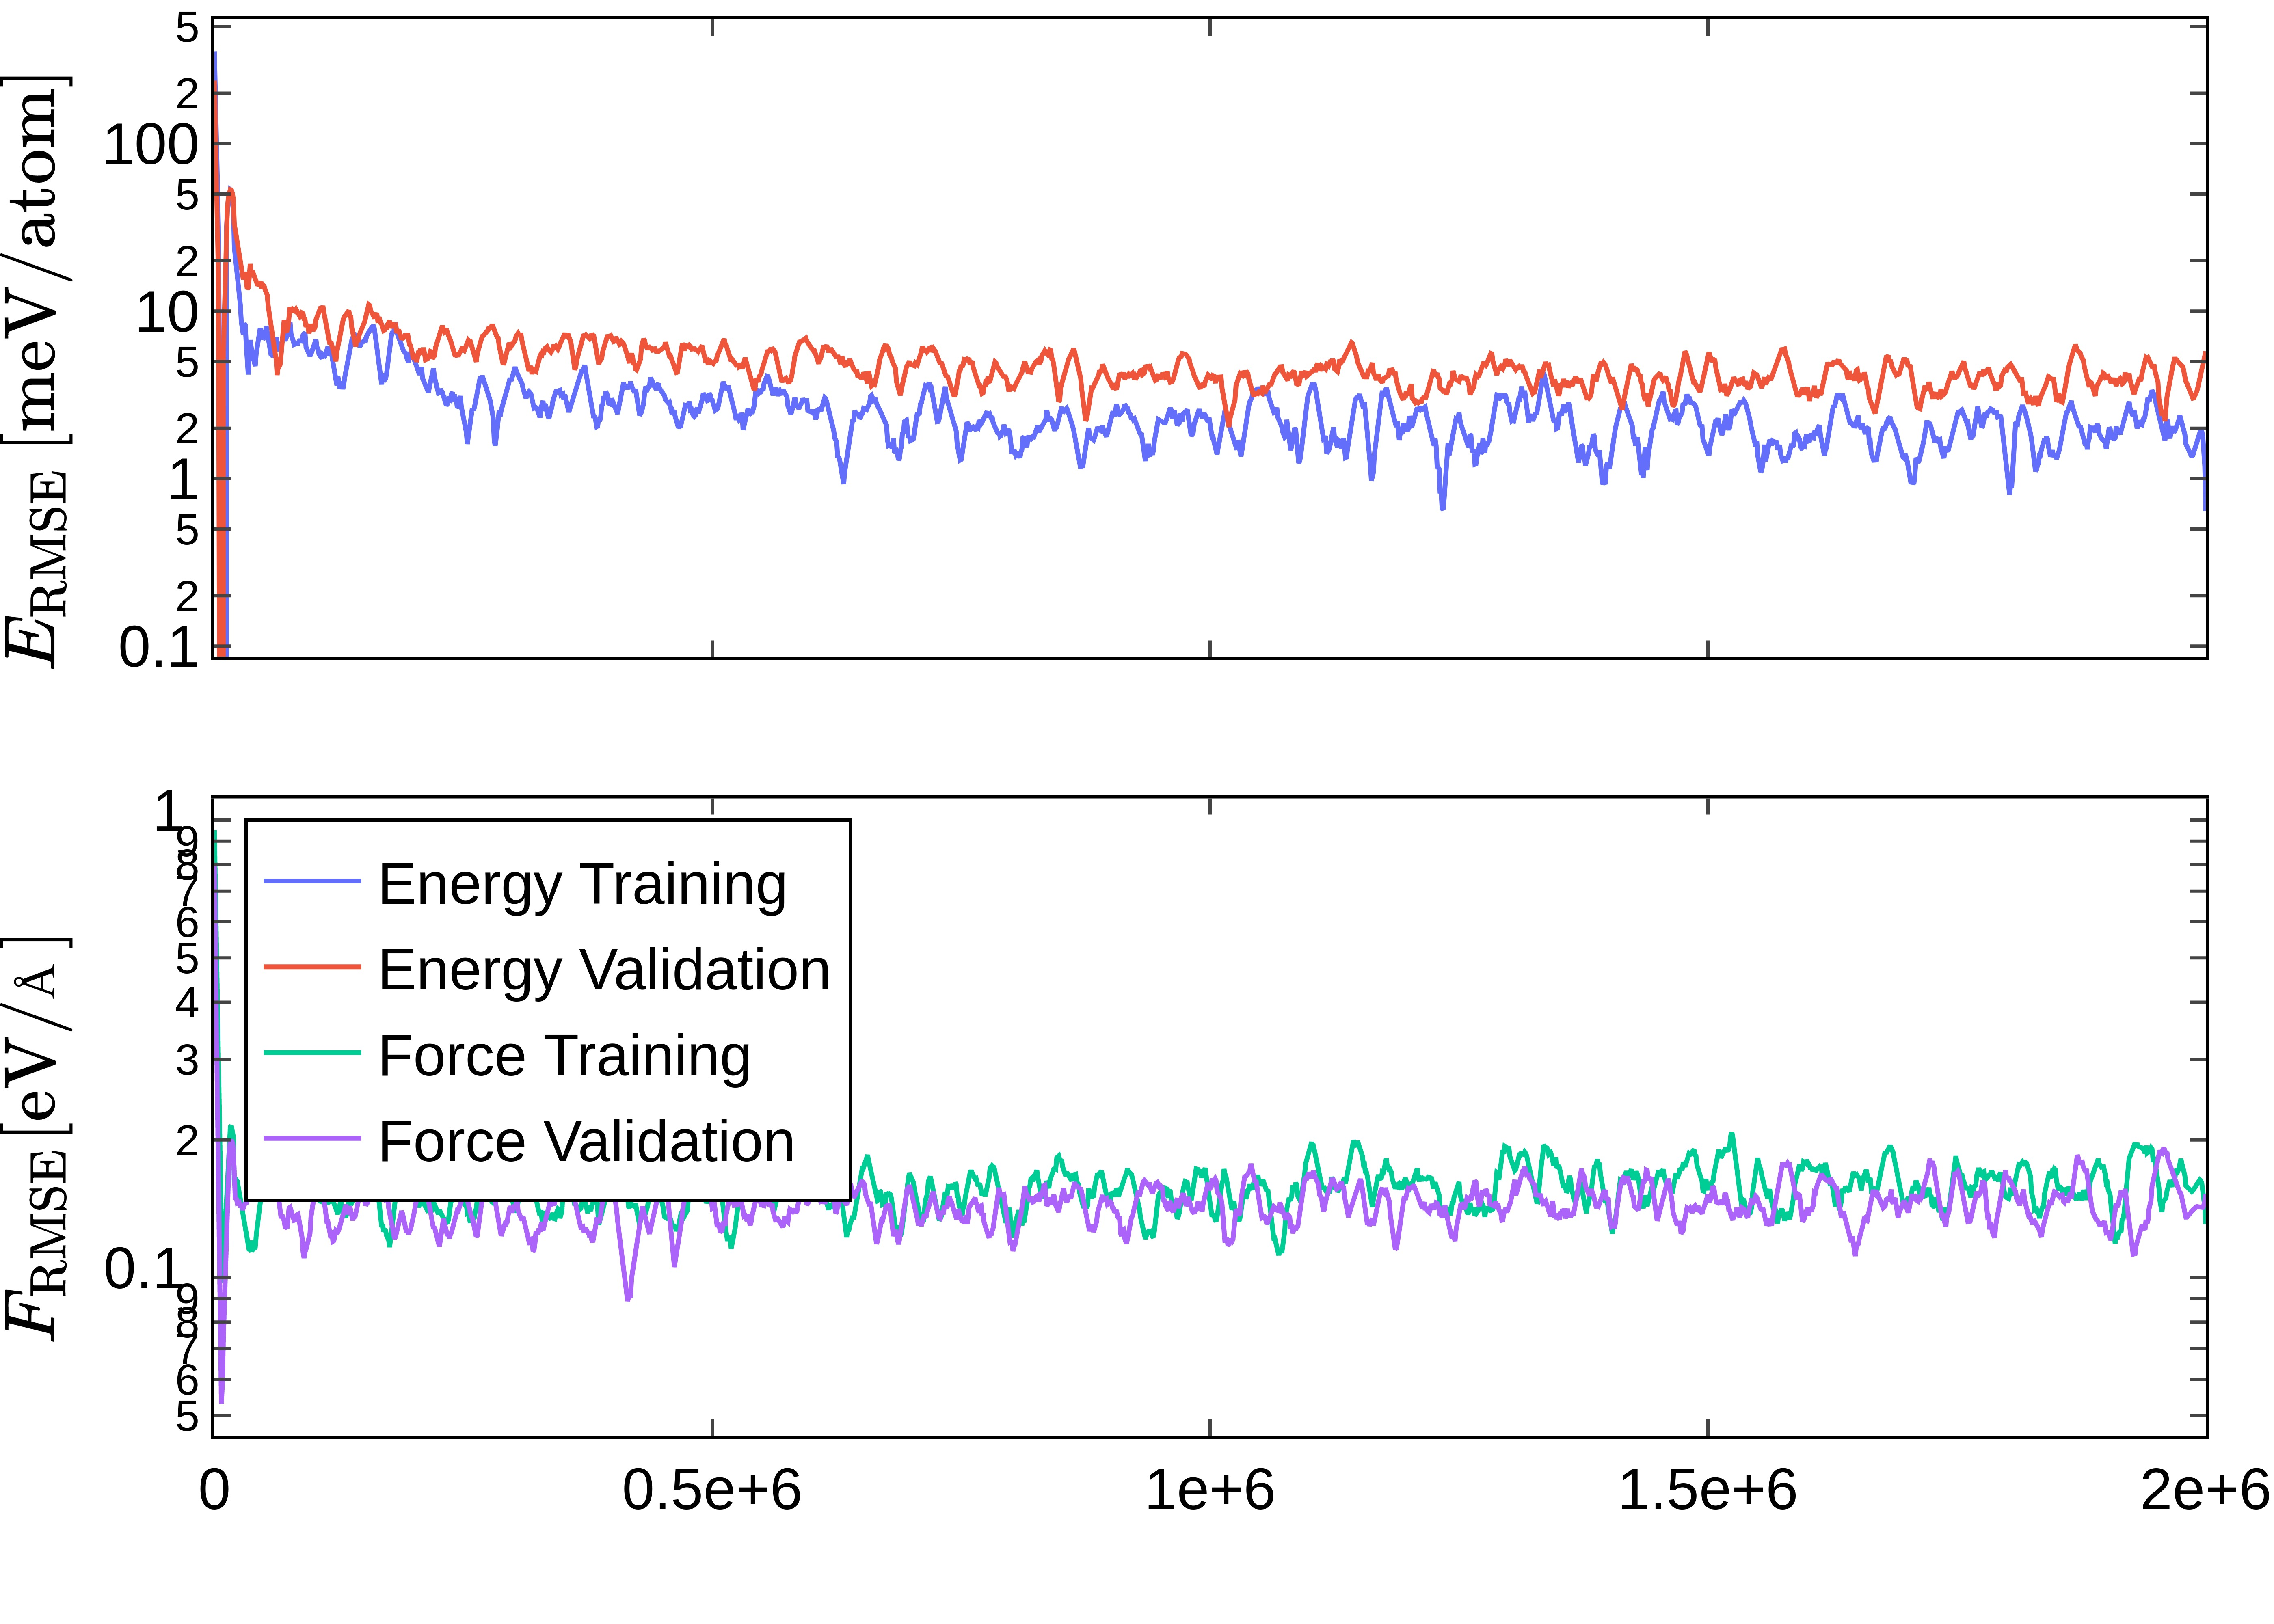
\includegraphics[width=.8\textwidth]{
      asset/crystalline_10,20,40d_10,10,10f_260222622s_energy_force_l_curve.jpg
    }
  \end{center}
  \caption{Learning curves for model \texttt{crystalline\_10,20,40d\_10,10,10f\_260222622s}.}
  \label{fig:crystalline_10,20,40d_10,10,10f_260222622s-learning-curves}
\end{figure}

\begin{figure}
  \begin{center}
    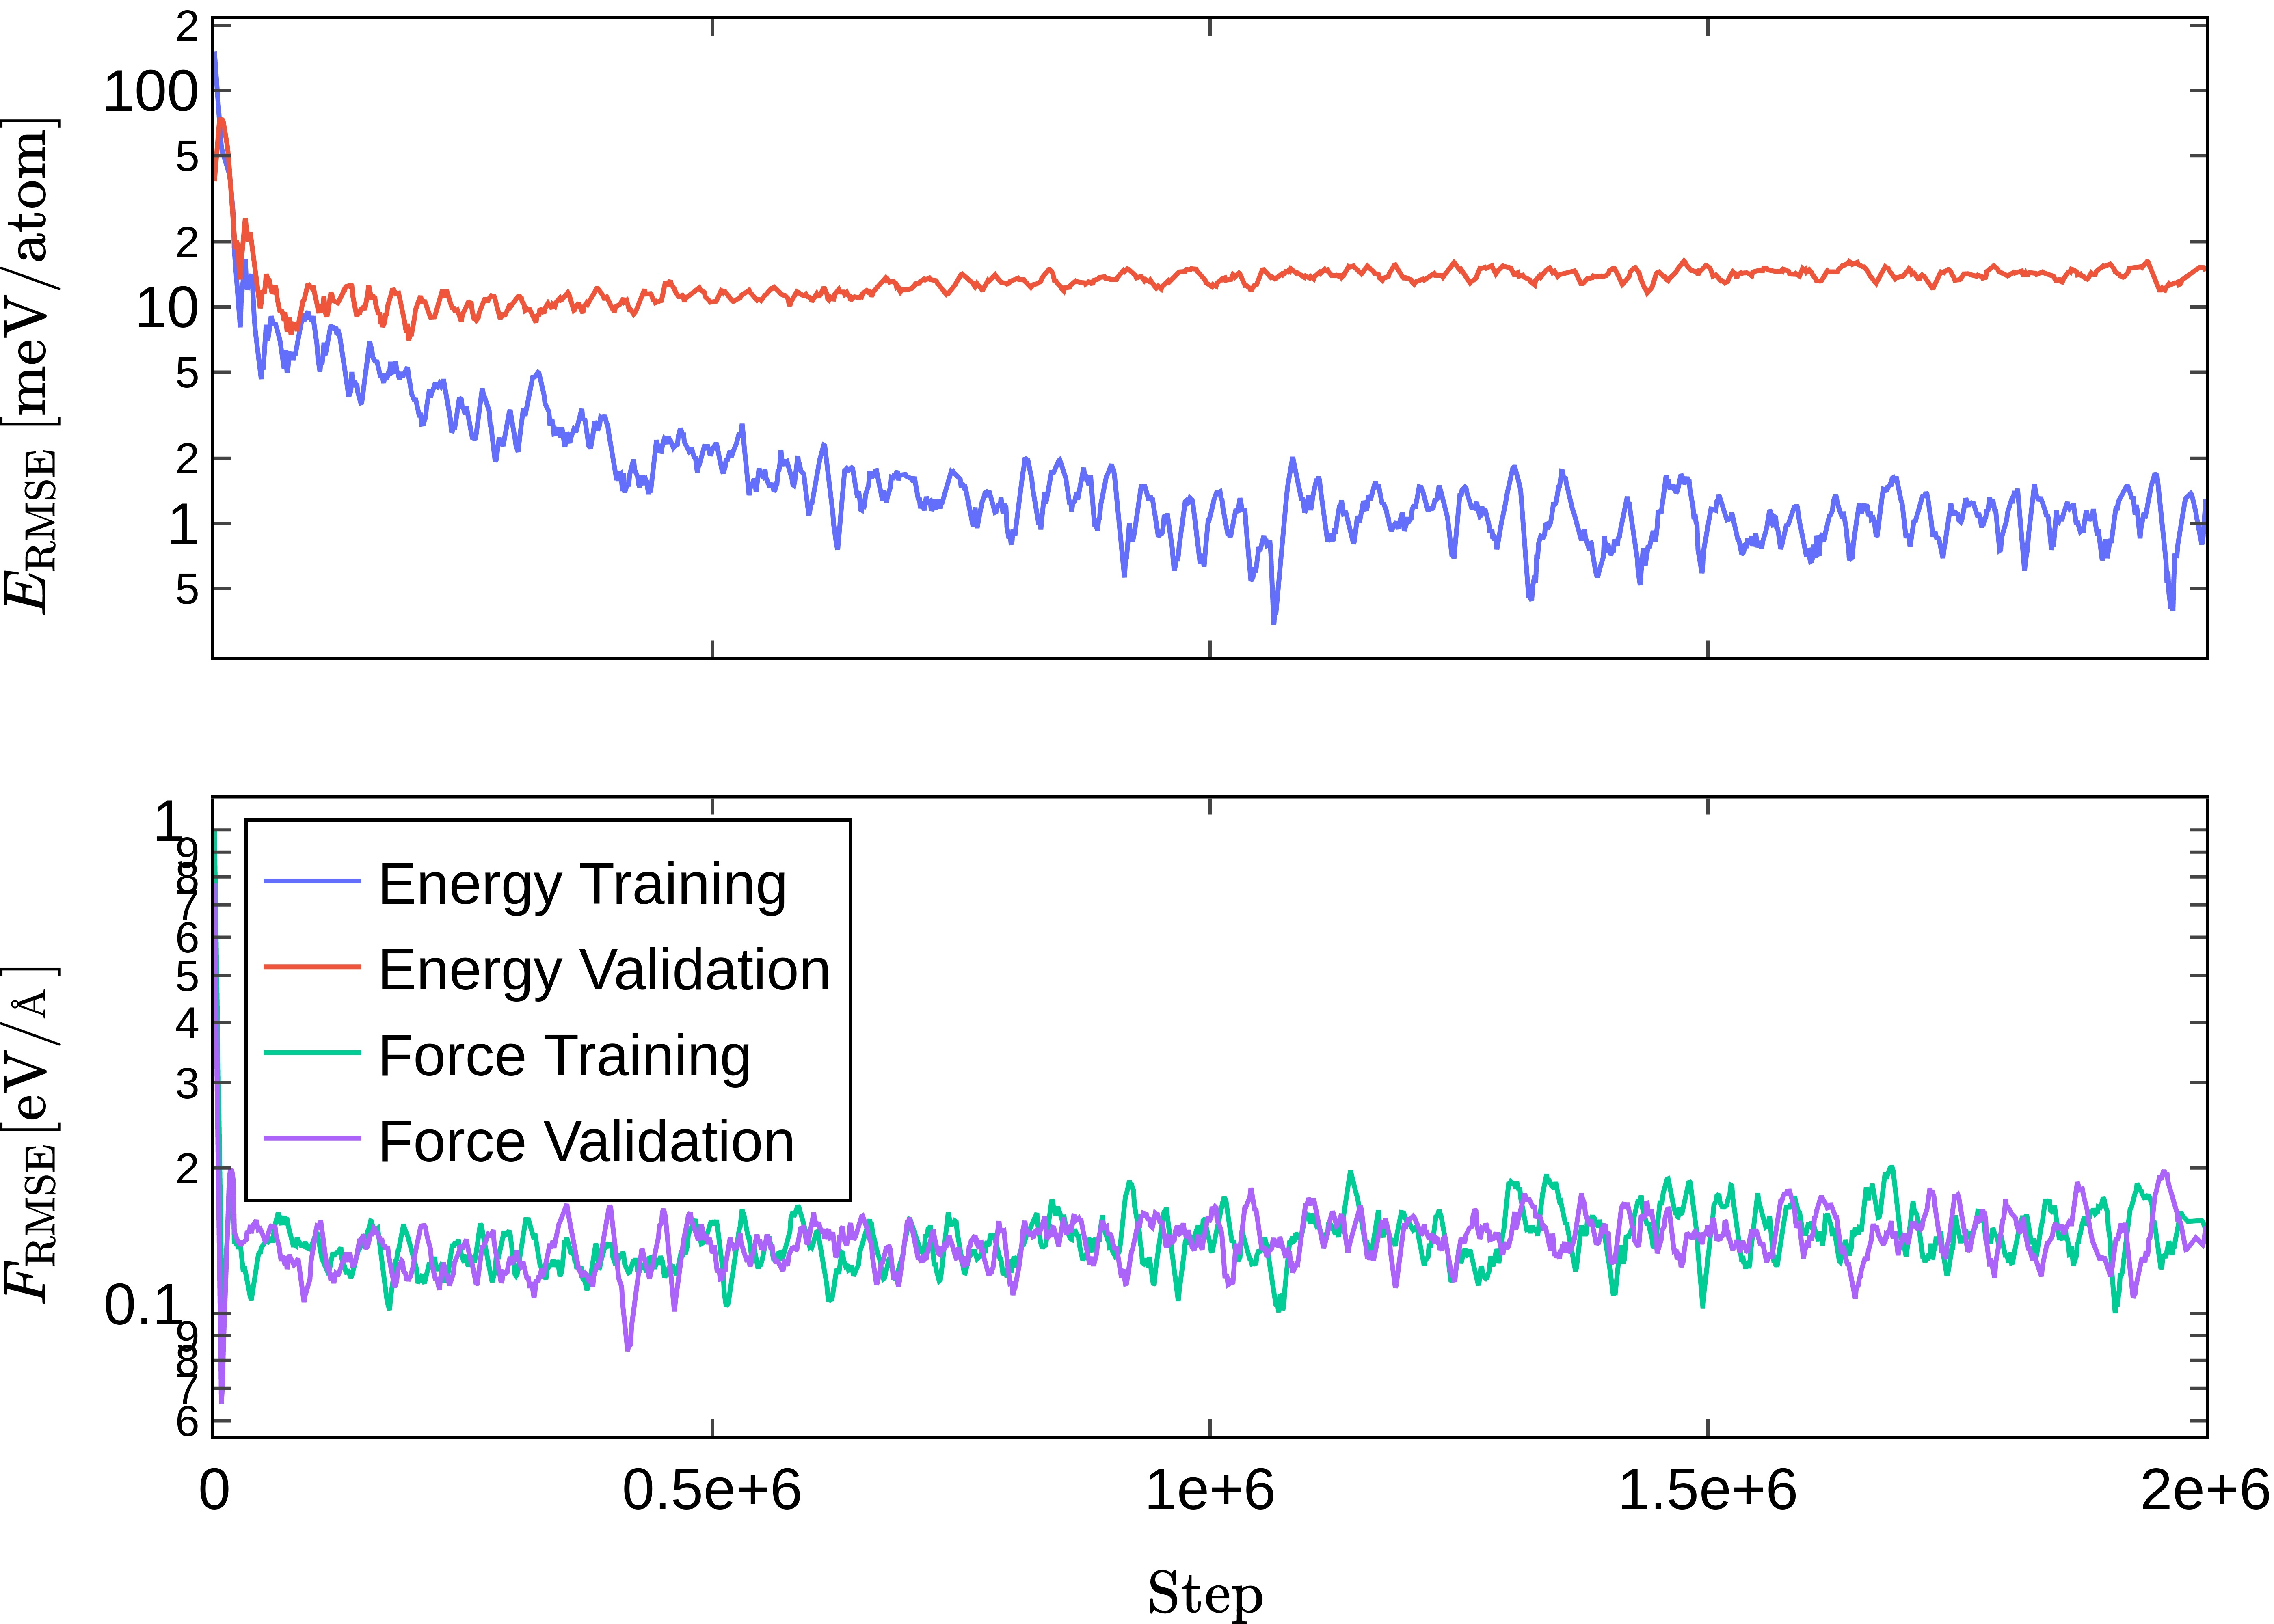
\includegraphics[width=.8\textwidth]{
      asset/crystalline_10,20,40d_75,75,75f_260222622s_energy_force_l_curve.jpg
    }
  \end{center}
  \caption{Learning curves for model \texttt{crystalline\_10,20,40d\_75,75,75f\_260222622s}.}
  \label{fig:crystalline_10,20,40d_75,75,75f_260222622s-learning-curves}
\end{figure}

\begin{figure}
  \begin{center}
    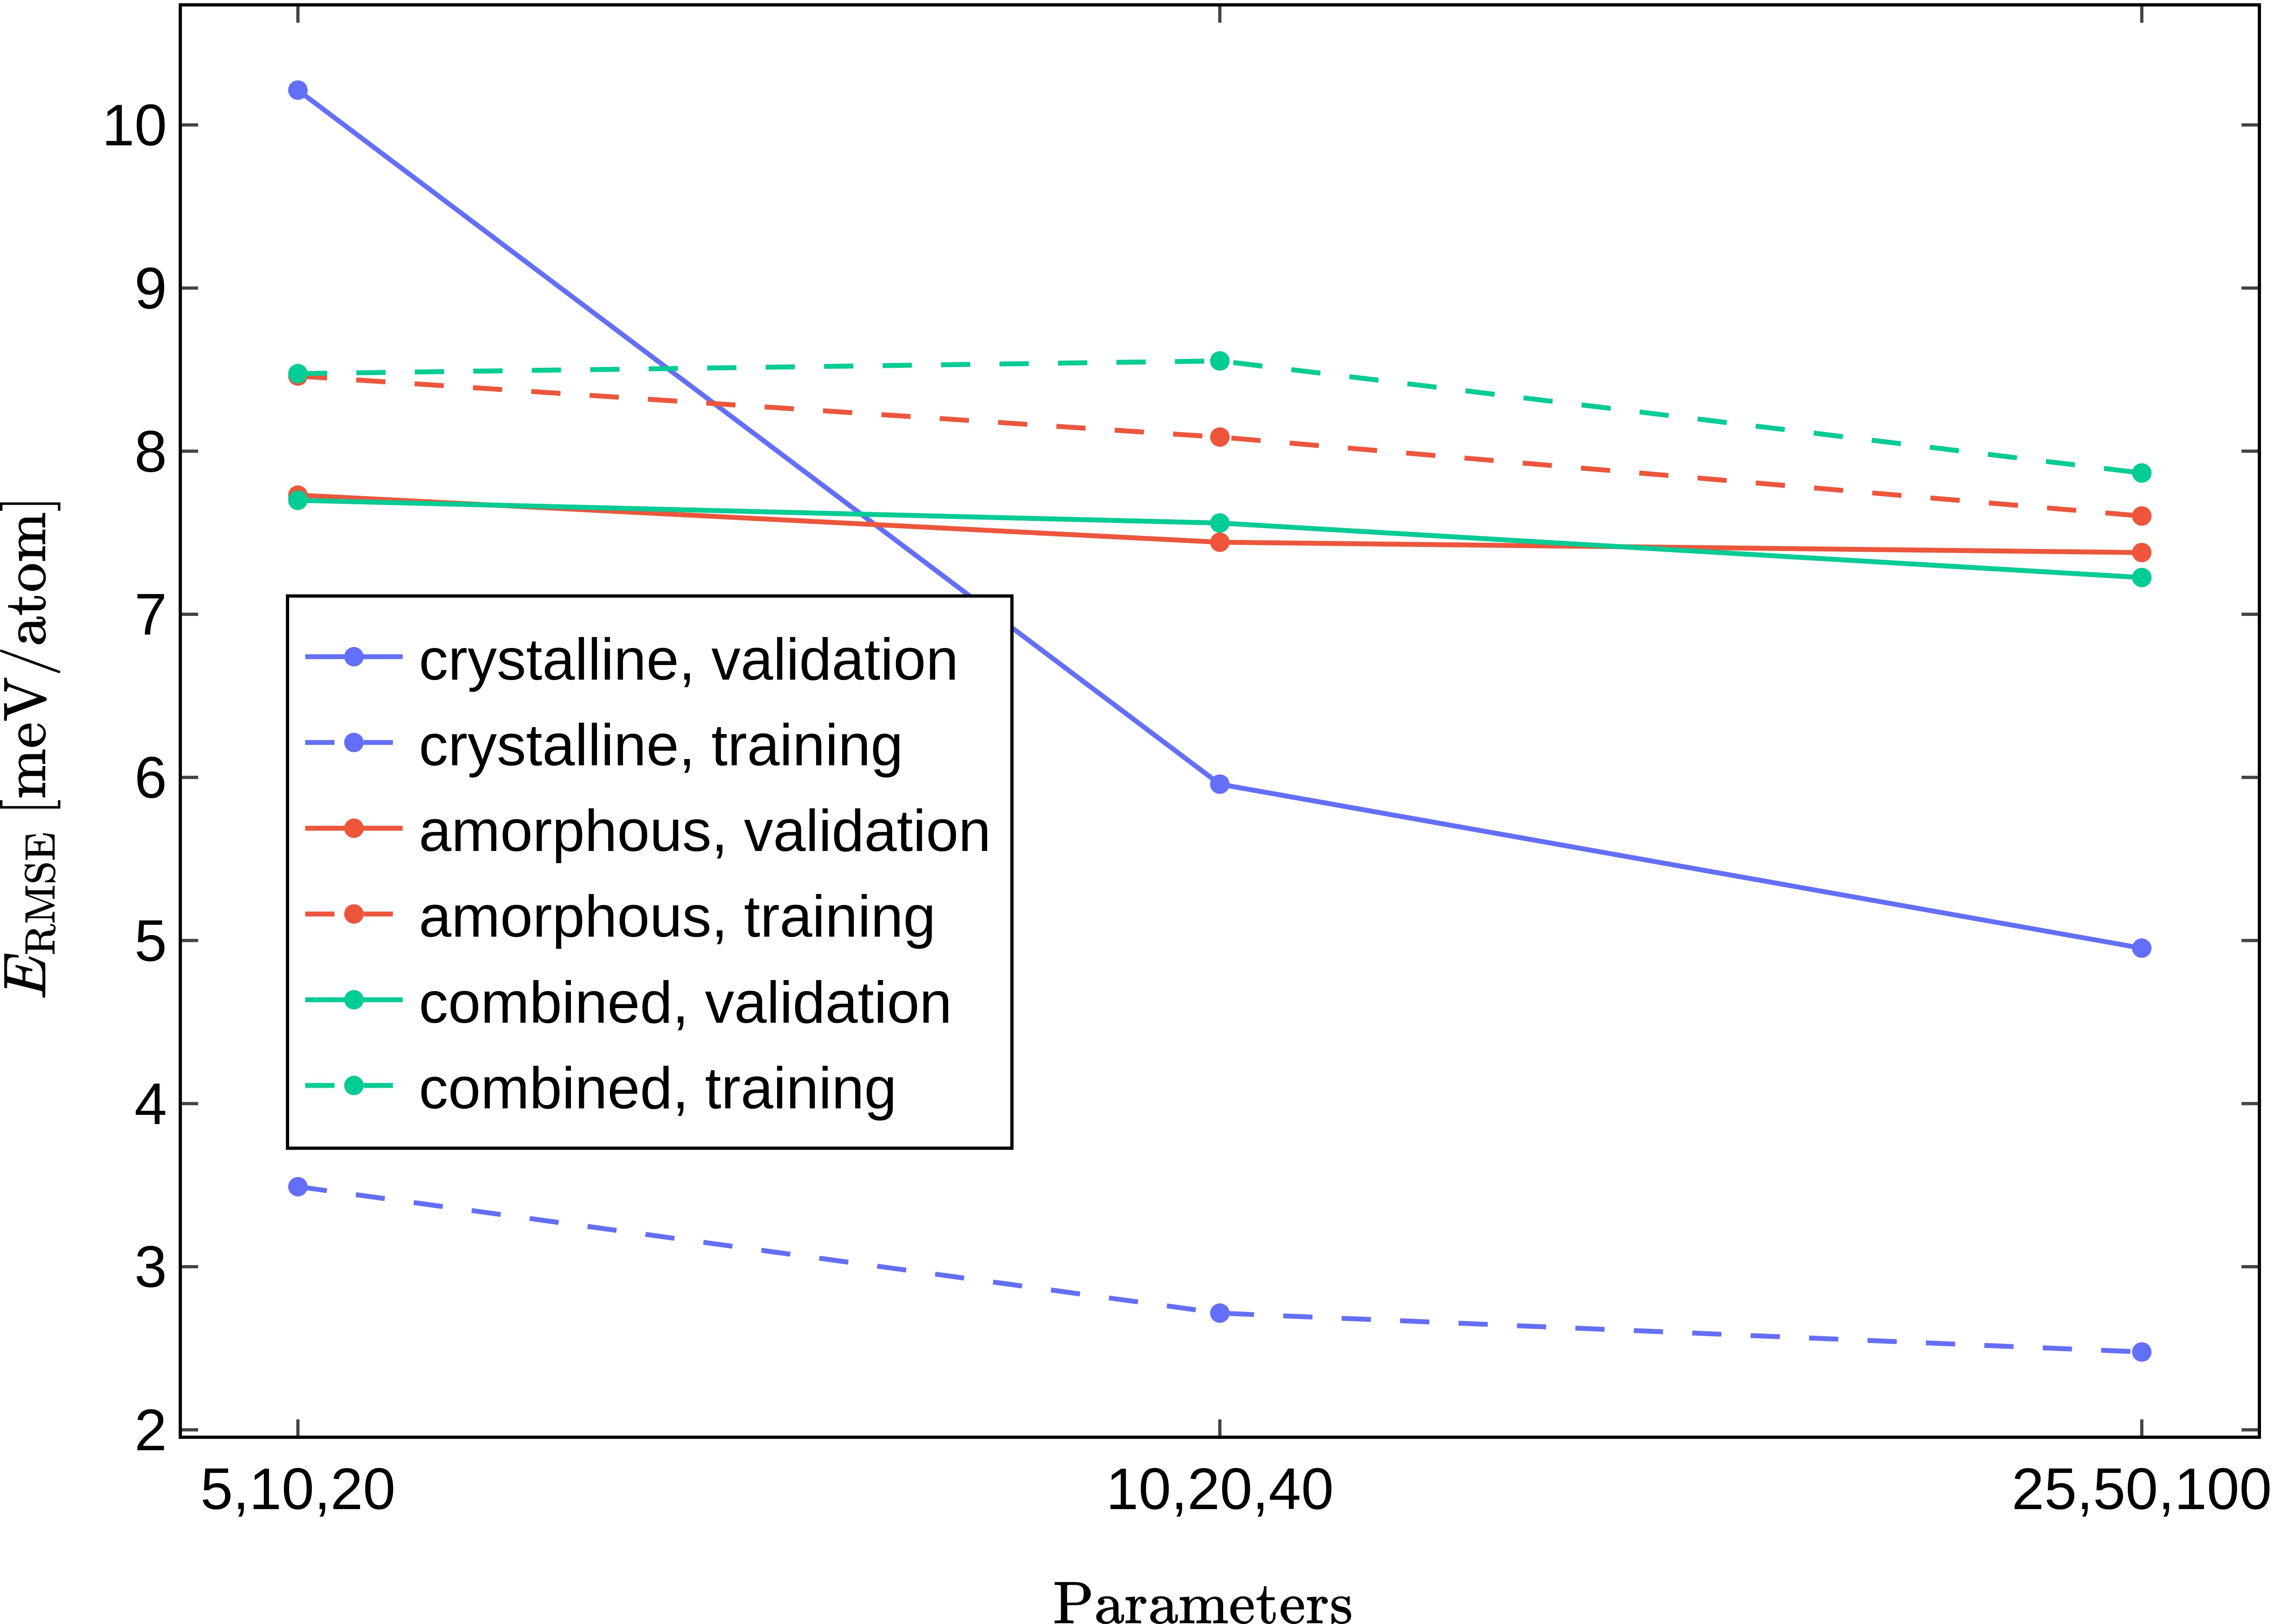
\includegraphics[width=.8\textwidth]{
      asset/descriptor_energy_error_evaluation.jpg
    }
  \end{center}
  \caption{Evaluation of energy errors for different descriptor neuron numbers.}
  \label{fig:descriptor_energy_error_evaluation}
\end{figure}

\begin{figure}
  \begin{center}
    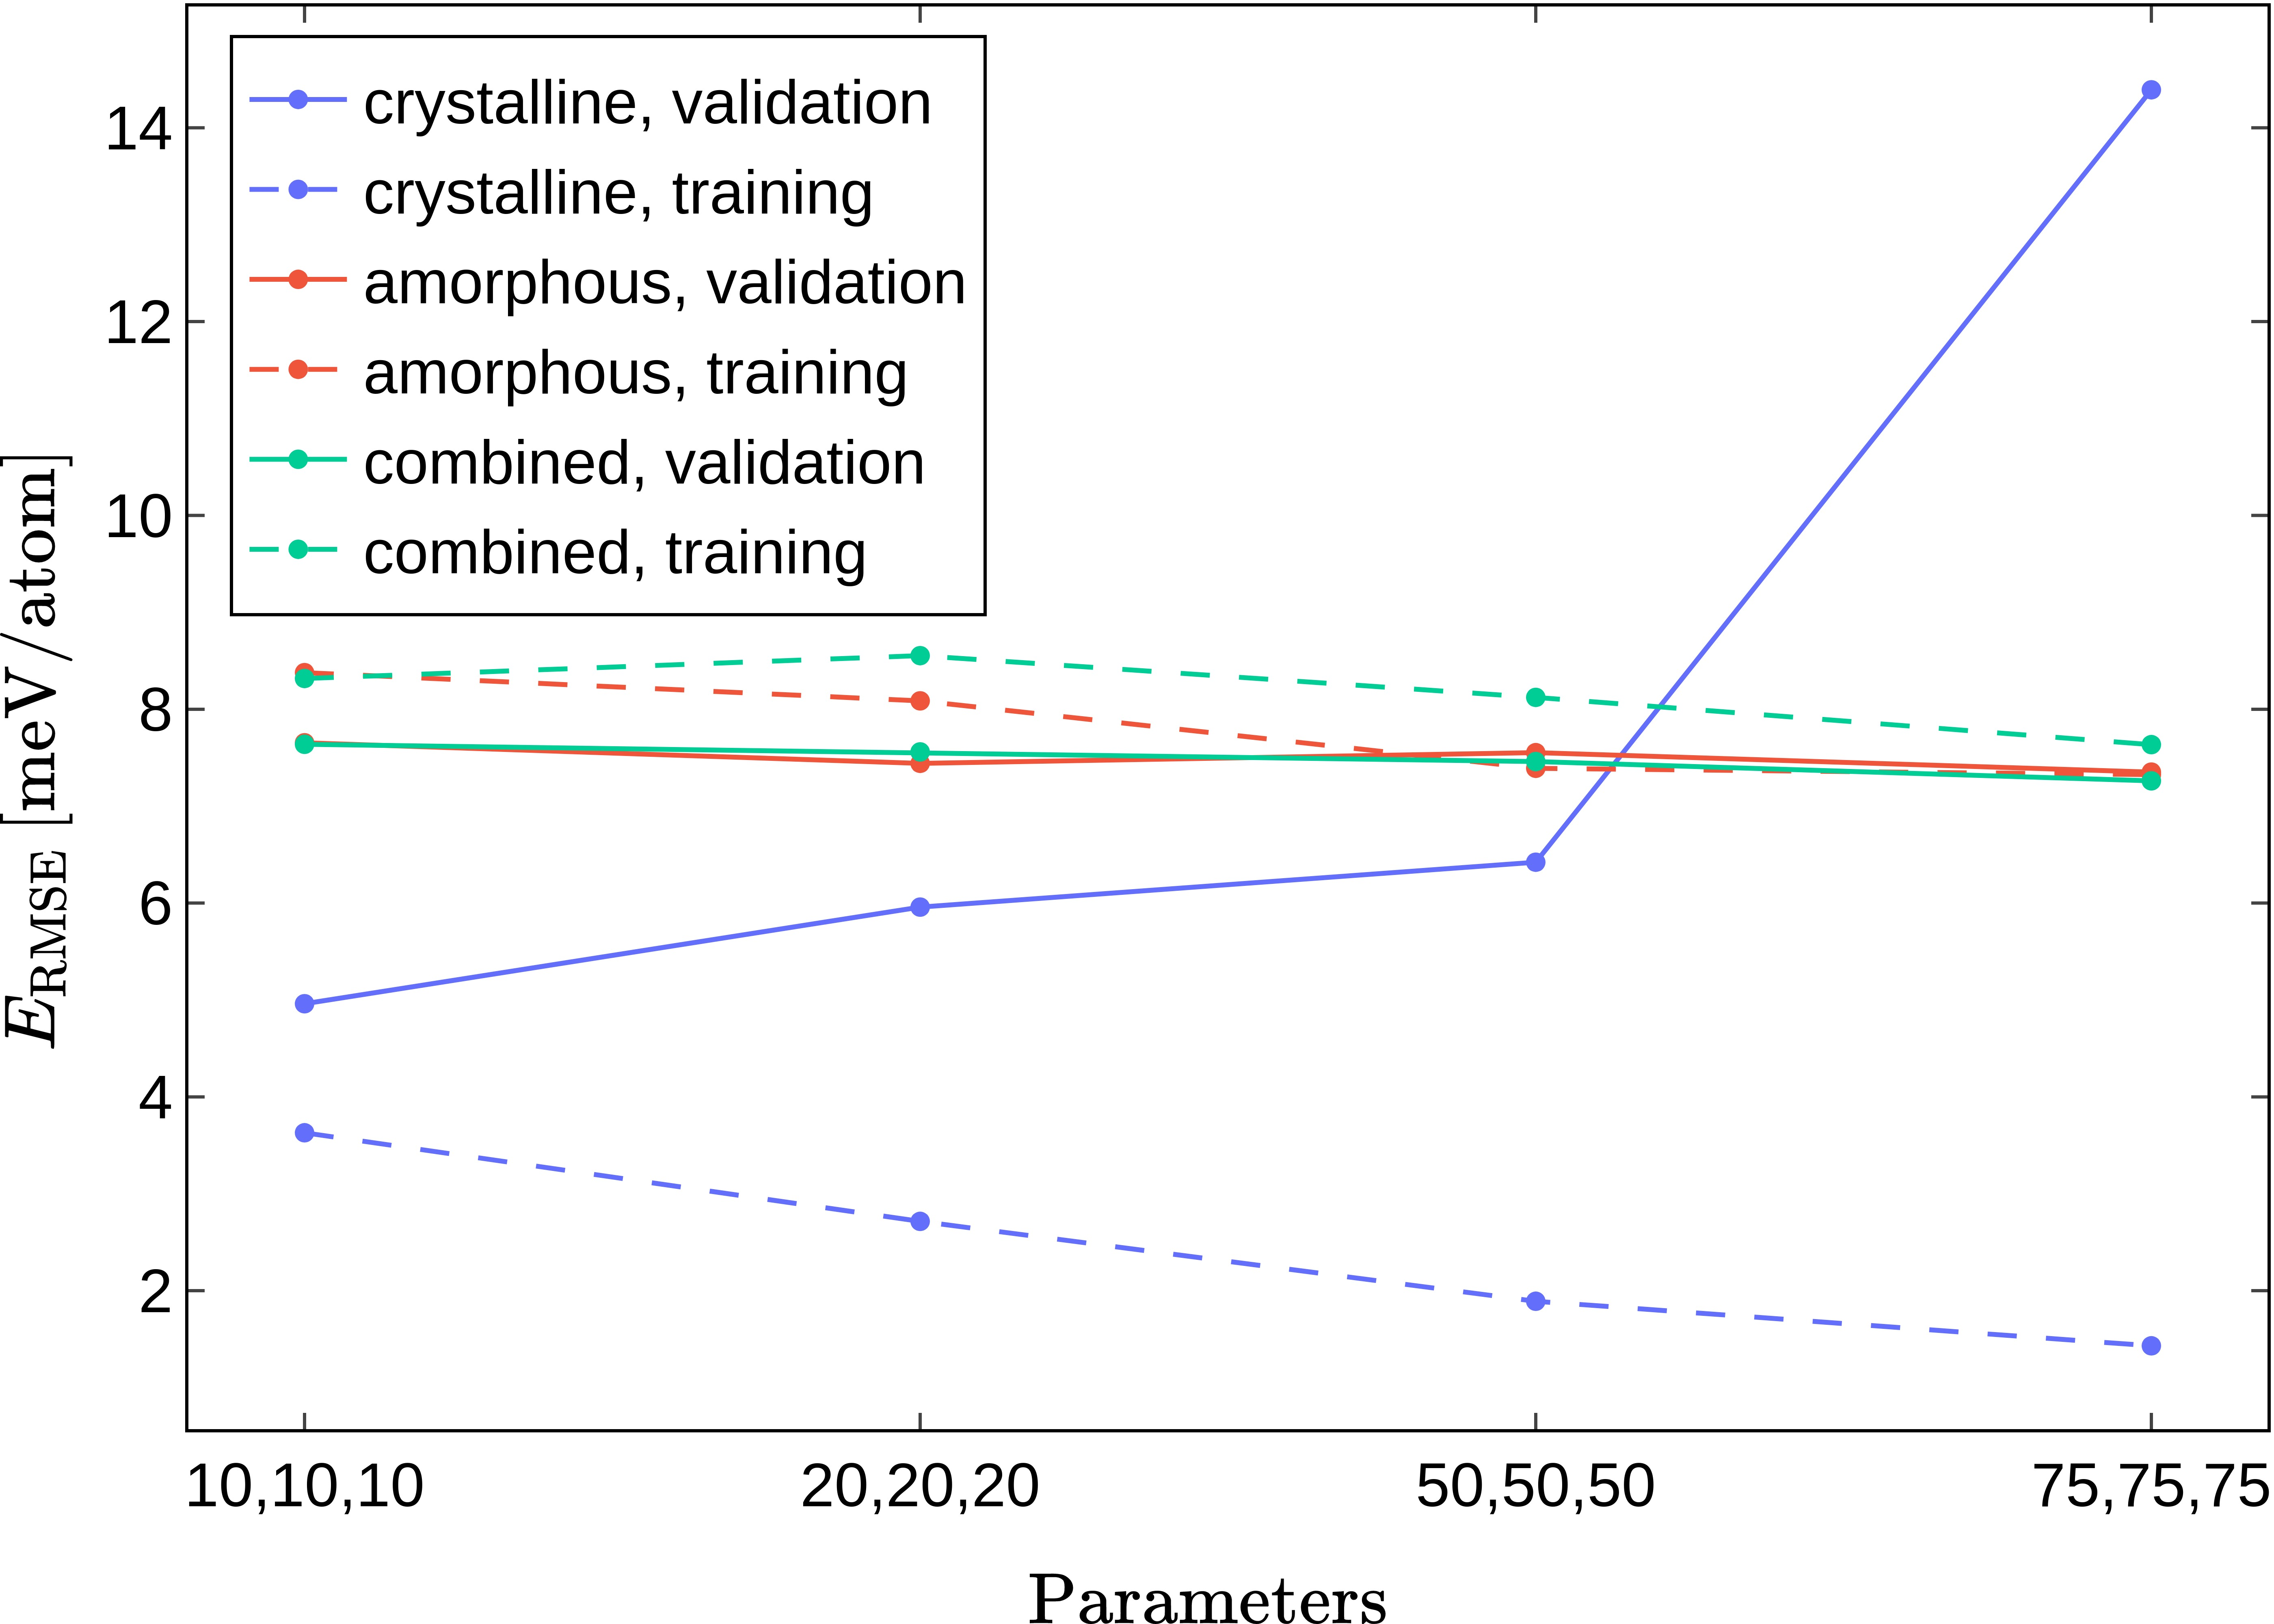
\includegraphics[width=.8\textwidth]{
      asset/fitting_energy_error_evaluation.jpg
    }
  \end{center}
  \caption{Evaluation of energy errors for different fitting neuron numbers.}
  \label{fig:fitting_energy_error_evaluation}
\end{figure}

\section{Inference Results}

The models \texttt{crystalline\_10,20,40d\_20,20,20f\_260222622s},\linebreak
\texttt{crystalline\_10,20,40d\_20,20,20f\_537693349s},\linebreak and
\texttt{crystalline\_10,20,40d\_20,20,20f\_836424474s} were used to calculate
relaxation volume and bulk modulus for the Si diamond crystalline structure
(cubic $\mathrm{F}\bar{\mathrm{d}}\mathrm{3m}$ space group). The inference
data with the fitted EOS models are shown below (figure
\ref{fig:crystalline_inference}). The calculated value for the relaxation
volume was $V_0 = 20.52 \pm 0.03$ \AA$^3$ and the calculated value for the
bulk modulus was
$B_{T_0} = 0.72 \pm 0.08 \, \mathrm{eV} \cdot \text{\AA}^{-3}$. Reference
materials for quantum mechanical calculations of the same structure give
values of $V_0 = 20.45617$ \AA$^3$ and
$B_{T_0} = 0.6121 \, \mathrm{eV} \cdot \text{\AA}^{-3}$\cite{osti_1190959}.

\begin{figure}
  \begin{center}
    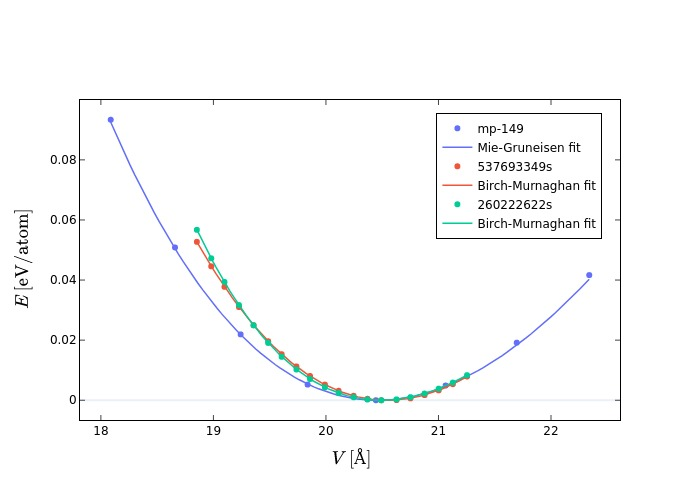
\includegraphics[width=.8\textwidth]{
      asset/crystalline_ev_curves.jpg
    }
  \end{center}
  \caption{Inference results for the Si diamond crystalline structure.}
  \label{fig:crystalline_inference}
\end{figure}
